% Options for packages loaded elsewhere
\PassOptionsToPackage{unicode}{hyperref}
\PassOptionsToPackage{hyphens}{url}
\PassOptionsToPackage{dvipsnames,svgnames,x11names}{xcolor}
%
\documentclass[
  table]{article}
\usepackage{amsmath,amssymb}
\usepackage{iftex}
\ifPDFTeX
  \usepackage[T1]{fontenc}
  \usepackage[utf8]{inputenc}
  \usepackage{textcomp} % provide euro and other symbols
\else % if luatex or xetex
  \usepackage{unicode-math} % this also loads fontspec
  \defaultfontfeatures{Scale=MatchLowercase}
  \defaultfontfeatures[\rmfamily]{Ligatures=TeX,Scale=1}
\fi
\usepackage{lmodern}
\ifPDFTeX\else
  % xetex/luatex font selection
\fi
% Use upquote if available, for straight quotes in verbatim environments
\IfFileExists{upquote.sty}{\usepackage{upquote}}{}
\IfFileExists{microtype.sty}{% use microtype if available
  \usepackage[]{microtype}
  \UseMicrotypeSet[protrusion]{basicmath} % disable protrusion for tt fonts
}{}
\makeatletter
\@ifundefined{KOMAClassName}{% if non-KOMA class
  \IfFileExists{parskip.sty}{%
    \usepackage{parskip}
  }{% else
    \setlength{\parindent}{0pt}
    \setlength{\parskip}{6pt plus 2pt minus 1pt}}
}{% if KOMA class
  \KOMAoptions{parskip=half}}
\makeatother
\usepackage{xcolor}
\usepackage{graphicx}
\makeatletter
\newsavebox\pandoc@box
\newcommand*\pandocbounded[1]{% scales image to fit in text height/width
  \sbox\pandoc@box{#1}%
  \Gscale@div\@tempa{\textheight}{\dimexpr\ht\pandoc@box+\dp\pandoc@box\relax}%
  \Gscale@div\@tempb{\linewidth}{\wd\pandoc@box}%
  \ifdim\@tempb\p@<\@tempa\p@\let\@tempa\@tempb\fi% select the smaller of both
  \ifdim\@tempa\p@<\p@\scalebox{\@tempa}{\usebox\pandoc@box}%
  \else\usebox{\pandoc@box}%
  \fi%
}
% Set default figure placement to htbp
\def\fps@figure{htbp}
\makeatother
\setlength{\emergencystretch}{3em} % prevent overfull lines
\providecommand{\tightlist}{%
  \setlength{\itemsep}{0pt}\setlength{\parskip}{0pt}}
\setcounter{secnumdepth}{-\maxdimen} % remove section numbering
% definitions for citeproc citations
\NewDocumentCommand\citeproctext{}{}
\NewDocumentCommand\citeproc{mm}{%
  \begingroup\def\citeproctext{#2}\cite{#1}\endgroup}
\makeatletter
 % allow citations to break across lines
 \let\@cite@ofmt\@firstofone
 % avoid brackets around text for \cite:
 \def\@biblabel#1{}
 \def\@cite#1#2{{#1\if@tempswa , #2\fi}}
\makeatother
\newlength{\cslhangindent}
\setlength{\cslhangindent}{1.5em}
\newlength{\csllabelwidth}
\setlength{\csllabelwidth}{3em}
\newenvironment{CSLReferences}[2] % #1 hanging-indent, #2 entry-spacing
 {\begin{list}{}{%
  \setlength{\itemindent}{0pt}
  \setlength{\leftmargin}{0pt}
  \setlength{\parsep}{0pt}
  % turn on hanging indent if param 1 is 1
  \ifodd #1
   \setlength{\leftmargin}{\cslhangindent}
   \setlength{\itemindent}{-1\cslhangindent}
  \fi
  % set entry spacing
  \setlength{\itemsep}{#2\baselineskip}}}
 {\end{list}}
\usepackage{calc}
\newcommand{\CSLBlock}[1]{\hfill\break\parbox[t]{\linewidth}{\strut\ignorespaces#1\strut}}
\newcommand{\CSLLeftMargin}[1]{\parbox[t]{\csllabelwidth}{\strut#1\strut}}
\newcommand{\CSLRightInline}[1]{\parbox[t]{\linewidth - \csllabelwidth}{\strut#1\strut}}
\newcommand{\CSLIndent}[1]{\hspace{\cslhangindent}#1}
\usepackage{multirow}
\usepackage{rotating}
\usepackage{authblk}
\renewcommand\Affilfont{\small}
\usepackage{booktabs}
\usepackage{lscape}
\usepackage{bookmark}
\IfFileExists{xurl.sty}{\usepackage{xurl}}{} % add URL line breaks if available
\urlstyle{same}
\hypersetup{
  colorlinks=true,
  linkcolor={Maroon},
  filecolor={Maroon},
  citecolor={Blue},
  urlcolor={blue},
  pdfcreator={LaTeX via pandoc}}

\author{}
\date{\vspace{-2.5em}}

\begin{document}

\begin{centering}

$ $

\vspace{0.1 cm}

\LARGE

{\bf Magnetic Resonance Imaging Data Phenotypes for the Parkinson's Progression Markers Initiative}

\vspace{1.0 cm}

\normalsize

Brian B Avants$^{1,2}$,
Leon Fonville$^{1}$,
Olivia Hampton$^{1}$,
Alexandra Reardon$^{1}$,
Andrew Stenger$^{1}$,
Xue Wang$^{1}$,
Nicholas J Tustison$^{2}$,
James R Stone$^{2}$,
Philip A Cook$^3$,
Barbara Marebwa$^4$,
Lana M Chahine$^5$,
Kathleen L Poston$^6$,
Kenneth Marek$^7$,
Lino Becerra$^{1}$,
Roger Gunn$^{1}$
for the Alzheimer's Disease Neuroimaging Initiative*


\vspace{0.25 cm}

\small

$^1$Invicro, Needham, MA, USA

$^2$Department of Radiology and Medical Imaging, University of Virginia, Charlottesville, VA, USA

$^3$Department of Radiology, Perelman School of Medicine at the University of Pennsylvania, Philadelphia, PA, USA

$^4$Parkinson's Research, The Michael J. Fox Foundation,  New York City, New York, USA

$^5$Department of Neurology, University of Pittsburgh, Pittsburgh, PA, USA

$^6$Department of Neurology, Stanford University, Palo Alto, CA, USA

$^7$Institute for Neurodegenerative Disorders, New Haven, CT, USA


\end{centering}

\vspace{2.2 cm}

\small

Corresponding author:\\
Brian B. Avants\\
\href{mailto:avants@grasp.cis.upenn.edu}{\nolinkurl{avants@grasp.cis.upenn.edu}}

\noindent

\rule{4cm}{0.4pt}

\footnotesize

*Data used in preparation of this article were obtained from the
Alzheimer's Disease Neuroimaging Initiative (ADNI) database
(adni.loni.usc.edu). As such, the investigators within the ADNI
contributed to the design and implementation of ADNI and/or provided
data but did not participate in analysis or writing of this report. A
complete listing of ADNI investigators can be found at:
\url{http://adni.loni.usc.edu/wp-content/uploads/how_to_apply/ADNI_Acknowledgement_List.pdf}

\newpage

\normalsize

\section{Abstract}\label{abstract}

The Parkinson's Progression Markers Initiative (PPMI)
\href{https://www.ppmi-info.org}{ppmi-info.org} delivers multiple
modality MRI (M3RI) and biomarker data for a comprehensive longitudinal
study of Parkinson's Disease (PD). These provide quantitative indices of
deep brain and cortical structure (T1-weighted MRI), microstructural
integrity of brain tissue (diffusion-weighted imaging) and resting brain
function (resting state functional MRI). Integrating and uniformly
analyzing M3RI alongside non-imaging biological and clinical data is
challenging due to the distinct nature of each modality. This study
systematically organizes these complex data into a structured format,
provides a PD-focused evaluation of the methodologies and evidence for
technical robustness of the approach. As of April 2024, the cohort
encompasses 841 idiopathic PD, 309 genetic PD, 1364 presymptomatic PD
and 240 control subjects at baseline with a follow-up period at a mean
of 2.05 years (interquartile range : 1.03-2.98 years). The study
continues to enroll new participants as well as acquire MRIs at
follow-up.

\section{Background \& Summary}\label{background-summary}

Parkinson's Disease (PD) is characterized by the progressive
accumulation of Lewy bodies, primarily composed of misfolded
alpha-synuclein, and appearing in the substantia nigra at an early stage
(\citeproc{ref-fearnleyAgeingParkinsonDisease1991}{Fearnley and Lees
1991}). The spread of this pathology correlates with both motor and
non-motor symptoms of PD, underscoring alpha-synuclein's pivotal role in
disease progression (\citeproc{ref-lee_mechanisms_2006}{Lee and
Trojanowski 2006}; \citeproc{ref-dickson_neuropathology_2009}{Dickson et
al. 2009}; \citeproc{ref-calabresi_alpha-synuclein_2023}{Calabresi et
al. 2023}). The synuclein seed amplification assay (SAA) significantly
advanced PD research by enabling in vivo confirmation for the first
time. The Parkinson's Progression Markers Initiative (PPMI) study
enhances this development by offering a dataset of subjects assessed
with SAA and multimodal MRI (M3RI), facilitating the monitoring of PD
progression and the impact of synucleinopathy on brain structure and
function (\citeproc{ref-shahnawaz_discriminating_2020}{Shahnawaz et al.
2020}; \citeproc{ref-siderowf_assessment_2023}{Siderowf et al. 2023}).
Table 1 defines key terms that may be unfamiliar to some readers.

Analyzing longitudinal M3RI in the PPMI study necessitates accessible
data representations for the PD research community. While each MRI
modality provides distinct insights, their combined analysis is
challenging due to the data's high dimensionality and computational
demands. Therefore, creating clear, accessible data representations is
crucial for advancing PD research and fostering new discoveries in
particular using multi-view data linking evidence of pathology, symptoms
and imaging (\citeproc{ref-nemmi_totally_2019}{Nemmi et al. 2019};
\citeproc{ref-tremblay_sex_2020}{Tremblay et al. 2020};
\citeproc{ref-markello_multimodal_2021}{Markello et al. 2021}).

The study utilizes the Advanced Normalization Tools X (ANTsX) ecosystem
to process PPMI MRI from 2010 to early 2024, focusing on T1-weighted,
diffusion-weighted, and resting-state functional MRI (sMRI, dMRI and
rsfMRI, respectively). The extended duration of data collection
underscores the necessity for robust processing techniques that manage
the resultant heterogeneity in images. ANTsX, leveraging decades of MRI
analysis expertise, employs advanced techniques and integrates open
science, deep learning, and machine learning for efficient multi-site
M3RI data processing (\citeproc{ref-avants_pediatric_2015}{B. B. Avants
et al. 2015}; \citeproc{ref-stone_functional_2020}{Stone et al. 2020};
\citeproc{ref-tustison_antsx_2021}{Tustison et al. 2021}).

To establish face validity, this study leverages not only PPMI M3RI, but
also the Alzheimer's Disease Neuroimaging Initiative (ADNI)
(\citeproc{ref-veitch2024alzheimer}{Veitch et al. 2024}) and traveling
subject data in three cohorts
(\citeproc{ref-hawco_longitudinal_2022}{Hawco et al. 2022};
\citeproc{ref-tanaka_multi-site_2021}{Tanaka et al. 2021};
\citeproc{ref-tong_reproducibility_2019}{Tong et al. 2019}). We analyze
these data collectively and uniformly to establish reliability
benchmarks and to demonstrate feasibility of consistent processing in
multi-site studies such as PPMI. Additionally, we exemplify statistical
models using PPMI data that are appropriate for unlocking key questions
relevant to biomarker-confirmed PD and related conditions.

Historically, MRI research on PD has primarily utilized T1-weighted
structural imaging (sMRI) to investigate neuroanatomical changes. A
consistent finding across these studies has been the identification of
early atrophy in mid-brain regions, particularly the substantia nigra
(\citeproc{ref-schwarz_t1-weighted_2011}{Schwarz et al. 2011};
\citeproc{ref-aquino_substantia_2014}{Aquino et al. 2014};
\citeproc{ref-ryman_mri_2020}{Ryman and Poston 2020};
\citeproc{ref-poston_substantia_2020}{Poston et al. 2020}).
Diffusion-weighted MRI (dMRI) has further enhanced our understanding by
allowing for the investigation of white matter microstructural integrity
which may be impacted not only in sporadic PD
(\citeproc{ref-peran_magnetic_2010}{Péran et al. 2010};
\citeproc{ref-owens-walton_worldwide_2024}{Owens-Walton et al. 2024})
but also in genetic PD (\citeproc{ref-tolosa_lrrk2_2020}{Tolosa et al.
2020}; \citeproc{ref-owens-walton_worldwide_2024}{Owens-Walton et al.
2024}). Similarly, resting state functional MRI (rsfMRI) has unveiled
alterations in network connectivity in PD patients, highlighting changes
in the functional integration and segregation of brain networks involved
in motor and cognitive functions
(\citeproc{ref-hacker_resting_2012}{Hacker et al. 2012};
\citeproc{ref-kim_abnormal_2017}{Kim et al. 2017};
\citeproc{ref-esposito_rhythm-specific_2013}{Esposito et al. 2013}).
Taken together, these findings suggest that PD impacts both the
structural and functional aspects of the brain. More integrative
research in PD (\citeproc{ref-menke_mri_2009}{Menke et al. 2009};
\citeproc{ref-markello_multimodal_2021}{Markello et al. 2021}) is needed
to determine the sequence of these changes and how they may relate to
alpha-synuclein and potential copathology or comorbidity
(\citeproc{ref-simuni_biological_2024}{Simuni et al. 2024}).

The present study extends previous foundations by providing standardized
imaging data phenotypes (IDPs) for PPMI with a particular emphasis on an
accessible tabular representation. The summary IDPs are computed with
\href{https://pypi.org/project/antspymm/}{ANTsPyMM v1.4.0} and depend on
standard anatomical and functional hierarchies that are well-established
in the field and consistently integrated in this work across modalities.
This approach supports investigations based on T1w structural imaging,
dMRI, and rsfMRI either independently or collectively. Importantly,
these imaging variables easily merge with the associated demographics,
SAA status, clinical data such as the Movement Disorder
Society-Sponsored Unified Parkinson's Disease Rating Scale (MDS-UPDRS)
(\citeproc{ref-disease_unified_2003}{Disease 2003}) and standard PPMI
DAT-SPECT summary measurements (\citeproc{ref-bega_clinical_2021}{Bega
et al. 2021}; \citeproc{ref-droby_aberrant_2022}{Droby et al. 2022}).
Through this integrative methodology, we aim to contribute to a deeper
understanding of PD, facilitating the development of more effective
diagnostic and therapeutic strategies and accelerating PD research.

\begin{table}

\caption{\label{tab:unnamed-chunk-2}Glossary of key terms used in this document.}
\centering
\begin{tabular}[t]{lp{10cm}lp{10cm}}
\toprule
Term & Definition\\
\midrule
Parkinson's disease & A progressive neurodegenerative
 disorder characterized by tremors,
 rigidity, bradykinesia, and postural
 instability (PD).\\
Idiopathic PD & PD without identifiable genetic or
 environmental factors.\\
Sporadic PD & No clear family history of PD, often
 assumed to be idiopathic.\\
Alpha-synuclein & A protein that plays a key role in the
 pathogenesis of Parkinson's disease,
 characterized by its tendency to
 misfold and aggregate into toxic
 fibrils that contribute to
 neurodegeneration.\\
SAA & Synuclein Amplification Assay, a
 laboratory test used to stratify
 subjects as either alpha-synuclein
 positive or negative.\\
\addlinespace
Prodromal & A period of time during which an
 individual experiences symptoms or
 warning signs of a disease before its
 full-blown onset.\\
MDS-UPDRS & Movement Disorder Society-Unified
 Parkinson's Disease Rating Scale, a
 standardized assessment tool for
 evaluating motor and non-motor symptoms
 of Parkinson's disease.\\
MOCA & Montreal Cognitive Assessment, a widely
 used screening test for detecting
 cognitive impairment.\\
REM & Rapid Eye Movement sleep, a stage of
 sleep characterized by vivid dreams and
 increased brain activity and associated
 with PD risk when resulting in abnormal
 motor behaviors such as acting out
 dreams.\\
LRRK2 & Leucine-rich repeat kinase 2, a gene
 associated with an increased risk of
 developing Parkinson's disease.\\
\addlinespace
GBA & Glucocerebrosidase, a gene associated
 with an increased risk of developing
 Parkinson's disease.\\
PIGD & Postural instability and gait
 disturbance, a subtype of Parkinson's
 disease characterized by postural
 instability and gait difficulties.\\
sMRI & Structural Magnetic Resonance Imaging,
 a type of (usually T1-weighted) MRI
 that provides detailed images of brain
 anatomy.\\
dMRI & Diffusion Magnetic Resonance Imaging, a
 type of MRI that measures the diffusion
 of water molecules in the brain,
 providing information on white matter
 tracts and brain connectivity.\\
rsfMRI & Resting-state functional Magnetic
 Resonance Imaging, a type of functional
 MRI that measures brain activity while
 a person is at rest, providing
 information on brain functional
 connectivity.\\
\addlinespace
Traveling subjects & Participants in a research study who
 undergo repeated assessments and
 evaluations at different locations or
 time points, often used to study
 accuracy and reproducibility of imaging
 data across scanners.\\
IDP & Imaging data phenotype, a summary
 measurement appropriate for
 representing and interpreting imaging
 data in tabular form.\\
\bottomrule
\end{tabular}
\end{table}

\section{Methods}\label{methods}

\subsection{MRI data collection}\label{mri-data-collection}

MRI data collection occurred between 2010 and an April 2024 cutoff date
for these data. Two phases of MRI collection occurred in PPMI; the first
collected sMRI and later dMRI as part of exploratory investigations. In
2020, a new phase of collection sought to improve both MRI quality and
consistency and expand the number of modalities collected. The sequences
used at each site are provided in detail at
(\citeproc{ref-avants_ppmi_2024}{B. Avants 2024}) and in the original
Laboratory of Neuroimaging (LONI) source data (described below in Data
Records). The ``phase'' of data collection is captured in the variable
\texttt{imaging\_protocol}. The PPMI data includes control subjects,
idiopathic (sporadic) PD subjects and genetic PD subjects characterized
by GBA, LRRK2, SNCA and PRKN mutations; the latter two groups appear
infrequently in this PPMI M3RI cohort. Additionally, presymptomatic
subjects comprise a substantial and growing portion of the cohort; these
are also characterized by genetic mutations and/or early risk factors
for PD (hyposmia or RBD)
(\citeproc{ref-siderowf_assessment_2023}{Siderowf et al. 2023}). Table 2
summarizes the cohort characteristics. In the following sections, we
focus on the PD cohort with SAA measurements as the presymptomatic
cohort is undergoing significant additional data collection.

\definecolor{black}{rgb}{0.0, 0.0, 0.0} 
\begin{sidewaystable}[!hbtp]
\begin{center}
\begin{small}
\color{black}
\begin{tabular}{llccccccrr}
\multicolumn{9}{c}{Table 2. Baseline PPMI IDP cohort. AR=at-risk; MSA = multi-system atrophy; OtherGen = other genetic; RBD = REM Sleep Behavior Disorder.}\\ 
\hline
\textbf{}&\textbf{CN}&\textbf{GenAR}&\textbf{SporadicAR}&\textbf{OtherGenPD}&\textbf{LRRK2PD}&\textbf{GBAPD}&\textbf{SporadicPD}&\\ 
\textbf{}&\textbf{(N=748)}&\textbf{(N=553)}&\textbf{(N=811)}&\textbf{(N=10)}&\textbf{(N=185)}&\textbf{(N=119)}&\textbf{(N=851)}&\multirow{-2}{*}{p}\\ 
\hline
age                &69.8 ±  9.8&62.3 ±  7.4&68.1 ±  5.6&49.9 ± 14.0&64.9 ±  8.5&62.2 ±  9.6&63.6 ±  9.2&< 0.001\\ 
Sex                &&&&&&&&< 0.001\\ 
 \hspace{0.5cm} Female         &356 (47.6\%)&331 (59.9\%)&400 (49.3\%)&2 (20.0\%)&98 (53.0\%)&54 (45.4\%)&308 (36.2\%)&\\ 
 \hspace{0.5cm} Male           &392 (52.4\%)&222 (40.1\%)&411 (50.7\%)&8 (80.0\%)&87 (47.0\%)&65 (54.6\%)&543 (63.8\%)&\\ 
race               &&&&&&&&< 0.001\\ 
 \hspace{0.5cm} Asian          &4 ( 0.5\%)& 0 ( 0.0\%)&3 ( 0.4\%)& 0 ( 0.0\%)&1 ( 0.5\%)& 0 ( 0.0\%)&14 ( 1.6\%)&\\ 
 \hspace{0.5cm} Black          &10 ( 1.3\%)& 0 ( 0.0\%)&6 ( 0.7\%)& 0 ( 0.0\%)& 0 ( 0.0\%)&2 ( 1.7\%)&11 ( 1.3\%)&\\ 
 \hspace{0.5cm} not.spec.      &507 (67.8\%)&6 ( 1.1\%)&8 ( 1.0\%)& 0 ( 0.0\%)& 0 ( 0.0\%)& 0 ( 0.0\%)&6 ( 0.7\%)&\\ 
 \hspace{0.5cm} Other          &8 ( 1.1\%)&12 ( 2.2\%)&27 ( 3.3\%)& 0 ( 0.0\%)&14 ( 7.6\%)&2 ( 1.7\%)&24 ( 2.8\%)&\\ 
 \hspace{0.5cm} White          &219 (29.3\%)&535 (96.7\%)&767 (94.6\%)&10 (100.0\%)&170 (91.9\%)&115 (96.6\%)&796 (93.5\%)&\\ 
duration.yrs       &   \hspace{0.5cm}& 0.8 ±  1.2&   \hspace{0.5cm}& 3.6 ±  3.7& 3.0 ±  2.1& 2.7 ±  1.9& 0.7 ±  0.6&< 0.001\\ 
updrs.totscore     & 4.8 ±  4.4& 9.5 ±  8.8&13.1 ± 10.4&33.1 ± 16.7&37.4 ± 17.7&45.5 ± 14.9&35.0 ± 15.1&< 0.001\\ 
CSFSAA             &&&&&&&&< 0.001\\ 
 \hspace{0.5cm} Negative       &474 (86.2\%)&484 (92.4\%)&127 (35.8\%)&4 (50.0\%)&61 (35.7\%)&6 ( 6.7\%)&49 ( 7.4\%)&\\ 
 \hspace{0.5cm} Positive       &76 (13.8\%)&39 ( 7.4\%)&226 (63.7\%)&4 (50.0\%)&109 (63.7\%)&82 (91.1\%)&608 (92.3\%)&\\ 
 \hspace{0.5cm} PosMSA         & 0 ( 0.0\%)&1 ( 0.2\%)&2 ( 0.6\%)& 0 ( 0.0\%)&1 ( 0.6\%)&2 ( 2.2\%)&2 ( 0.3\%)&\\ 
LEDD               & 0.0 ±  0.0& 4.1 ± 45.8& 0.4 ± 10.5&573.2 ± 450.4&465.0 ± 425.7&542.3 ± 551.3& 9.9 ± 62.6&< 0.001\\ 
subgroup           &&&&&&&&< 0.001\\ 
 \hspace{0.5cm} GBA            & 0 ( 0.0\%)&281 (50.8\%)& 0 ( 0.0\%)& 0 ( 0.0\%)& 0 ( 0.0\%)&119 (100.0\%)& 0 ( 0.0\%)&\\ 
 \hspace{0.5cm} GBA + RBD      & 0 ( 0.0\%)&1 ( 0.2\%)& 0 ( 0.0\%)& 0 ( 0.0\%)& 0 ( 0.0\%)& 0 ( 0.0\%)& 0 ( 0.0\%)&\\ 
 \hspace{0.5cm} Healthy Control&242 (100.0\%)& 0 ( 0.0\%)& 0 ( 0.0\%)& 0 ( 0.0\%)& 0 ( 0.0\%)& 0 ( 0.0\%)& 0 ( 0.0\%)&\\ 
 \hspace{0.5cm} Hyposmia       & 0 ( 0.0\%)& 0 ( 0.0\%)&567 (69.9\%)& 0 ( 0.0\%)& 0 ( 0.0\%)& 0 ( 0.0\%)& 0 ( 0.0\%)&\\ 
 \hspace{0.5cm} LRRK2          & 0 ( 0.0\%)&245 (44.3\%)& 0 ( 0.0\%)& 0 ( 0.0\%)&178 (96.2\%)& 0 ( 0.0\%)& 0 ( 0.0\%)&\\ 
 \hspace{0.5cm} LRRK2 + GBA    & 0 ( 0.0\%)&24 ( 4.3\%)& 0 ( 0.0\%)& 0 ( 0.0\%)&7 ( 3.8\%)& 0 ( 0.0\%)& 0 ( 0.0\%)&\\ 
 \hspace{0.5cm} PRKN           & 0 ( 0.0\%)& 0 ( 0.0\%)& 0 ( 0.0\%)&5 (50.0\%)& 0 ( 0.0\%)& 0 ( 0.0\%)& 0 ( 0.0\%)&\\ 
 \hspace{0.5cm} RBD            & 0 ( 0.0\%)& 0 ( 0.0\%)&244 (30.1\%)& 0 ( 0.0\%)& 0 ( 0.0\%)& 0 ( 0.0\%)&2 ( 0.2\%)&\\ 
 \hspace{0.5cm} SNCA           & 0 ( 0.0\%)&2 ( 0.4\%)& 0 ( 0.0\%)&5 (50.0\%)& 0 ( 0.0\%)& 0 ( 0.0\%)& 0 ( 0.0\%)&\\ 
 \hspace{0.5cm} Sporadic PD    & 0 ( 0.0\%)& 0 ( 0.0\%)& 0 ( 0.0\%)& 0 ( 0.0\%)& 0 ( 0.0\%)& 0 ( 0.0\%)&849 (99.8\%)&\\ 
imaging.protocol   &&&&&&&&< 0.001\\ 
 \hspace{0.5cm} ADNI           &506 (67.6\%)& 0 ( 0.0\%)& 0 ( 0.0\%)& 0 ( 0.0\%)& 0 ( 0.0\%)& 0 ( 0.0\%)& 0 ( 0.0\%)&\\ 
 \hspace{0.5cm} PPMI1          &169 (22.6\%)&538 (97.3\%)&60 ( 7.4\%)&3 (30.0\%)&172 (93.0\%)&110 (92.4\%)&388 (45.6\%)&\\ 
 \hspace{0.5cm} PPMI2          &73 ( 9.8\%)&15 ( 2.7\%)&751 (92.6\%)&7 (70.0\%)&13 ( 7.0\%)&9 ( 7.6\%)&463 (54.4\%)&\\ 
\hline
\end{tabular}
\end{small}
\end{center}
\end{sidewaystable}
\color{black}

\subsubsection{Data Organization}\label{data-organization}

Raw DICOM data was downloaded from LONI and converted to nifti format
via \texttt{dcm2niix} (\citeproc{ref-li_first_2016}{Li et al. 2016}).
These data were then organized into a directory tree following the
\href{https://github.com/stnava/biomedicalDataOrganization}{NRG format}
illustrated in Figure 1. This BIDS-like structure
(\citeproc{ref-gorgolewski_brain_2016}{Gorgolewski et al. 2016}) is
defined to aid in longitudinal analyses of multiple modality data and
intends to support: (a) sortable and specific dates associated with
imaging sessions; (b) links between the data on disk and its origin
(LONI) through the ``Image ID''; (c) easy maintenance of multiple
modality data collections; and (d) predictable input/output structure.
Critically, the unique ID allows the original data associated with an
IDP to be easily found in LONI. In brief, this system assigns each image
-- and categories of derivative data -- a directory and individual file
name that assist in making data findable, accessible, interpretable and
reproducible (FAIR) for both early and downstream processing.

\begin{figure}
\centering
\pandocbounded{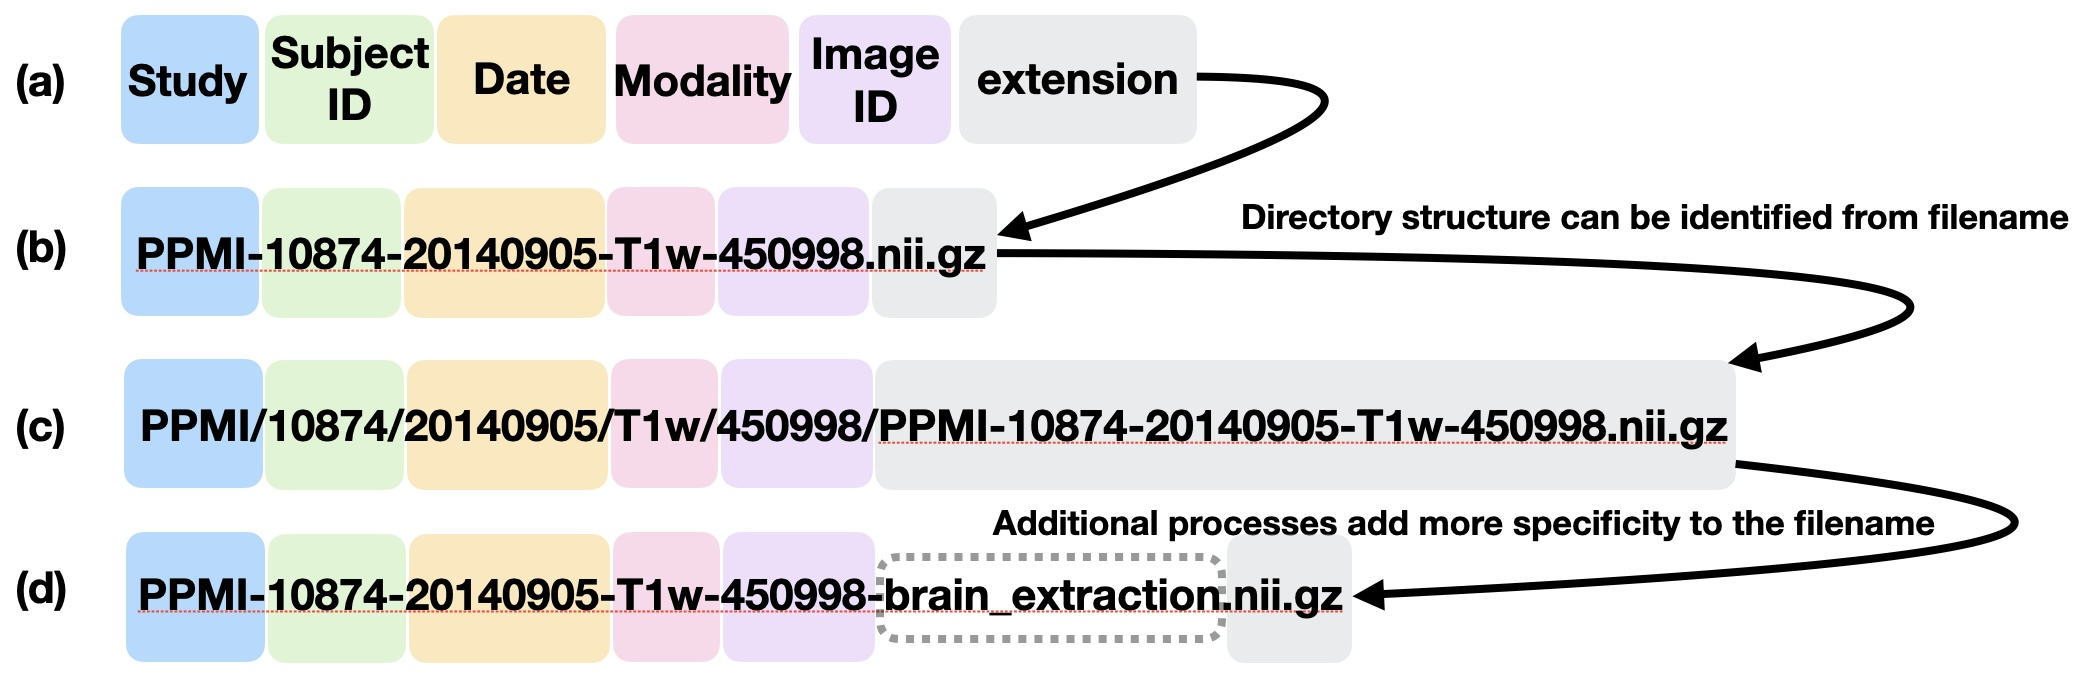
\includegraphics[keepaspectratio]{../figs/nrg_format.jpg}}
\caption{The NRG format supports predictable and interpretable data
storage and processing that can easily be tied back to the LONI source
DICOM. The filename proceeds from less specific information (Project ID
at reader's left) to the most specific (unique image ID at reader's
right). A specific character -- here the dash -- is reserved exclusively
as a separator between the stages of information.}
\end{figure}

\subsubsection{ANTsPyMM processing}\label{antspymm-processing}

ANTsPyMM collects and documents best ANTsX practices for both data
inspection and IDP generation for the modalities of interest in a single
Python package. While ANTsPyMM supports BIDS format, it behaves most
predictably and safely with NRG format. Each ``run'' of the integrated
multiple modality processing encoded by ANTsPyMM is driven by a data
frame that defines a multiple modality ``collection'' of images for a
given subject at a given date. There are two key functions that aid
users in defining the appropriate input data structure and sending that
data to processing. The first is
\texttt{antspymm.generate\_mm\_dataframe} which generates the
appropriate multiple modality subject dataframe that documents on disk
locations for image sets. The resulting dataframe defines the expected
input as well as output structures. The second key function runs the
multiple modality processing (\texttt{antspymm.mm\_csv}) based on the
multiple modality subject dataframe. The ``Usage Notes'' section
provides more details on this system with an accompanying reproducible
example based on freely accessible multiple modality neuroimaging.

\begin{figure}
\centering
\pandocbounded{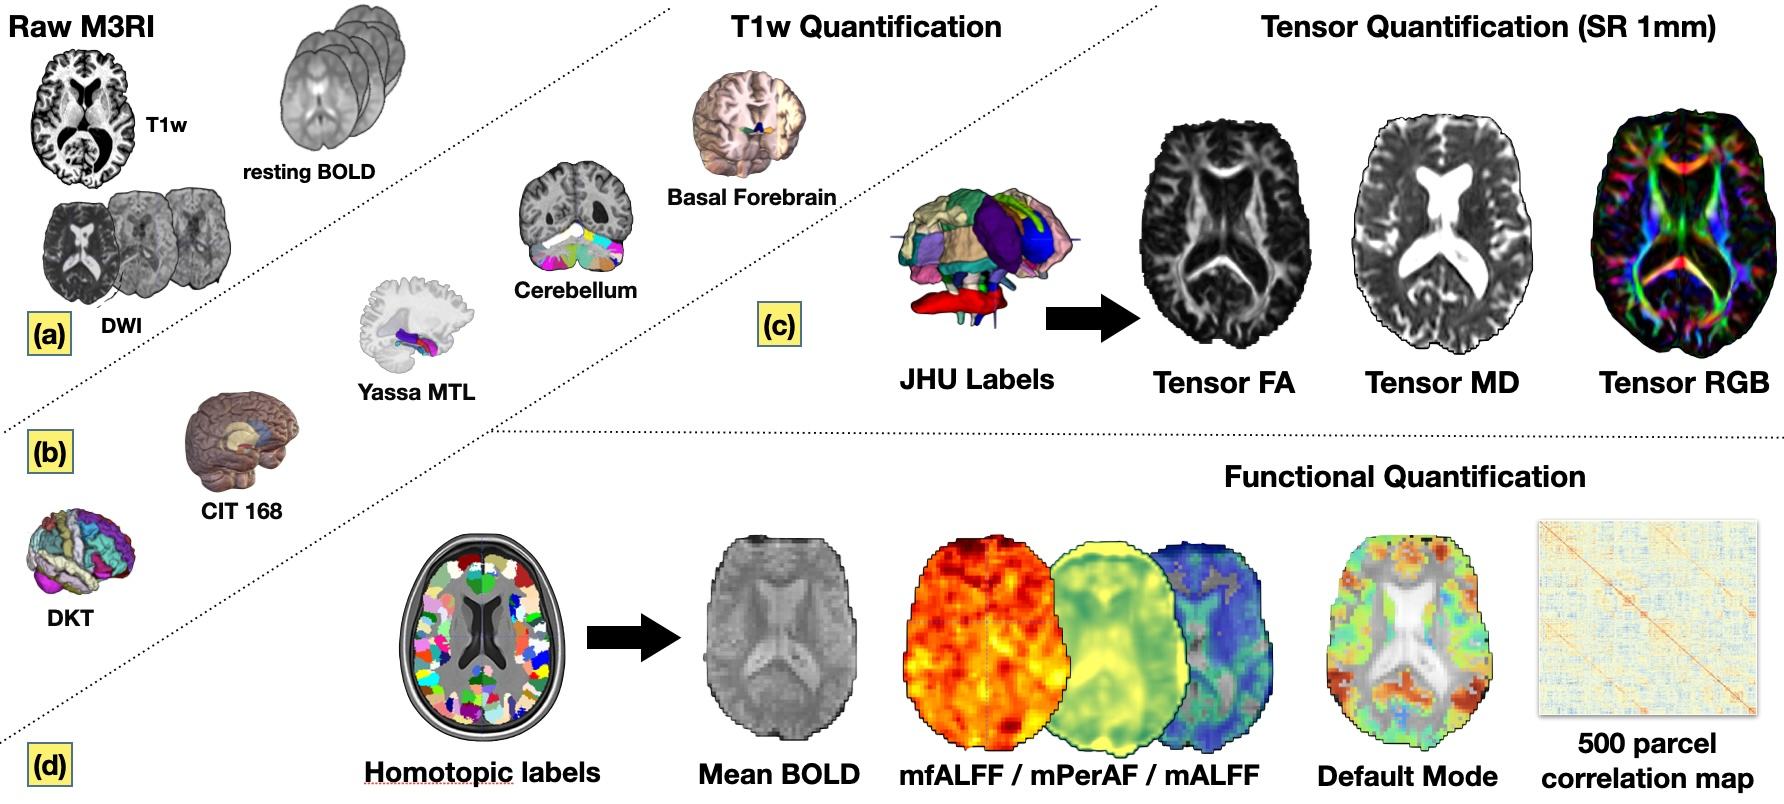
\includegraphics[keepaspectratio]{../figs/antspymm_3.jpg}}
\caption{Overview of ANTsPyMM outputs for T1-weighted MRI, diffusion MRI
and resting state fMRI. Panel (a) shows example input data; the package
does not require all modalities to be present -- only T1w. It also
handles arterial spin labeling (perfusion), FLAIR and neuromelanin, not
covered here. Panel (b) illustrates core T1w outputs across several
inter-related and PD relevant systems in the brain. Panel (c) shows the
standard outputs associated with dMRI. Whole brain tractography is also
output but no evaluation results are available to contextualize its
performance and, as such, we do not recommend its use. Panel (d)
summarizes the various rsfMRI outputs for processing parameter set
number 129 referred to with a prefix \texttt{rsfMRI\_fcnxpro129}.}
\end{figure}

\subsubsection{Semi-automated quality
assessment}\label{semi-automated-quality-assessment}

ANTsPyMM's primary goal is reliable M3RI IDP generation. Of necessity,
it also addresses quality control (QC) with particular focus on the T1w
modality i.e.~the core anatomical image that represents the most
consistently collected MRI in PPMI. T1w is the focus of QC because
ancillary modality processing depends heavily on anatomical labels
(e.g.~tissue segmentation, cortical parcellation) derived from these
images. As such, we developed an automated (deep learning based) T1w
reviewer that is trained on human (BA) QC reviews. Each T1w image is
therefore reviewed internally in the first stage of ANTsPyMM processing
by this \texttt{resnetGrader} (a deep learning model trained to predict
image quality) (\citeproc{ref-avants2023.02.02.23285376}{B. Avants et
al. 2023}). The grader will abort processing if the T1w does not achieve
a given baseline level of quality. Human visual inspection was performed
on images that pass the grader by BA and serves as a sanity check to the
automated method. The \texttt{resnetGrader} successfully filtered
unusable data and we selected a quality cutoff at 1.02 to filter out low
quality images. Similarly, the rsfMRI and dMRI were reviewed in post hoc
fashion. This process involved visually inspecting each estimated FA
image and each estimated default mode network connectivity map and its
associated mean BOLD image. Particular focus was paid to cases with high
motion and/or low SNR; such images were excluded from statistical
analyses.

\subsection{Neuroanatomical coordinate
systems}\label{neuroanatomical-coordinate-systems}

The statistical interpretation of processed images is aided by automatic
anatomic labeling with pre-specified coodinate systems or maps overlaid
on each subject's neuroimage. We leverage a recent homotopic
parcellation (\citeproc{ref-yan_homotopic_2023}{Yan et al. 2023}), the
Desikan-Killiany-Tourville (DKT) system
(\citeproc{ref-klein_101_2012}{Klein and Tourville 2012}), the CIT168
atlas (\citeproc{ref-pauli_high-resolution_2018}{Pauli, Nili, and Tyszka
2018}), the Johns Hopkins University (JHU) white matter labels
(\citeproc{ref-mori_white_2009}{Mori, Oishi, and Faria 2009}), the
Schmahmann cerebellar parcellation
(\citeproc{ref-lyu_multimodal_2024}{Lyu et al. 2024};
\citeproc{ref-carass_comparing_2018}{Carass et al. 2018}), brain stem
labels (\citeproc{ref-iglesias_bayesian_2015}{Iglesias et al. 2015}), a
medial temporal lobe schema (\citeproc{ref-rizvi_posterior_2023-1}{Rizvi
et al. 2023}) and labels derived from probabilistic maps of the basal
forebrain (\citeproc{ref-liu_nucleus_2015}{Liu et al. 2015};
\citeproc{ref-zaborszky_stereotaxic_2008}{Zaborszky et al. 2008}). These
systems are described in detail in online
\href{http://htmlpreview.github.io/?https://github.com/stnava/ANTsPyMM/blob/main/docs/make_dict_table.html}{data
dictionary and associated documentation} for this project. These
coordinate system enable PD researchers to interrogate a variety of
hypotheses related to, for example, known functional networks,
association hubs, cholinergic networks, the striatum or dopaminergic
systems.

\subsubsection{Structural MRI
processing}\label{structural-mri-processing}

T1-weighted MRI processing is described in detail in
(\citeproc{ref-tustison_antsx_2023}{Tustison et al. 2023},
\citeproc{ref-tustison_antsx_2021}{2021}). This open-source software
ecosystem includes tools for image registration, segmentation, and
super-resolution (SR) as customized for the human brain. The derived
measurements are tabulated by the neuroanatomical coordinates defined
above and include cortical and subcortical measurements and
morphological measurements of the hippocampus, basal forebrain and
cerebellum. The results of this stage are key to consistent processing
of rsfMRI and dMRI. We provide both original resolution (OR) and SR
results as part of this effort. For SR processing of sMRI, the network
is applied -- first -- over the whole head sMRI image to double
resolution along all axes within the brain parenchyma. Otherwise, SR and
OR processing are identical. SR training with 3D perceptual losses is
documented in the \texttt{Python} package
\href{https://pypi.org/project/siq/}{siq} and is based on
\texttt{tensorflow} implementations of a volumetric deep back projection
network (DBPN) (\citeproc{ref-avants2023.02.02.23285376}{B. Avants et
al. 2023}; \citeproc{ref-tustison_antsx_2021}{Tustison et al. 2021};
\citeproc{ref-haris_deep_2020}{Haris, Shakhnarovich, and Ukita 2020}) .
See Figure 2 for examples of these outputs. IDPs derived from the sMRI
processing are denoted by prefixes \texttt{T1w} and \texttt{T1Hier}.

\begin{figure}
\centering
\pandocbounded{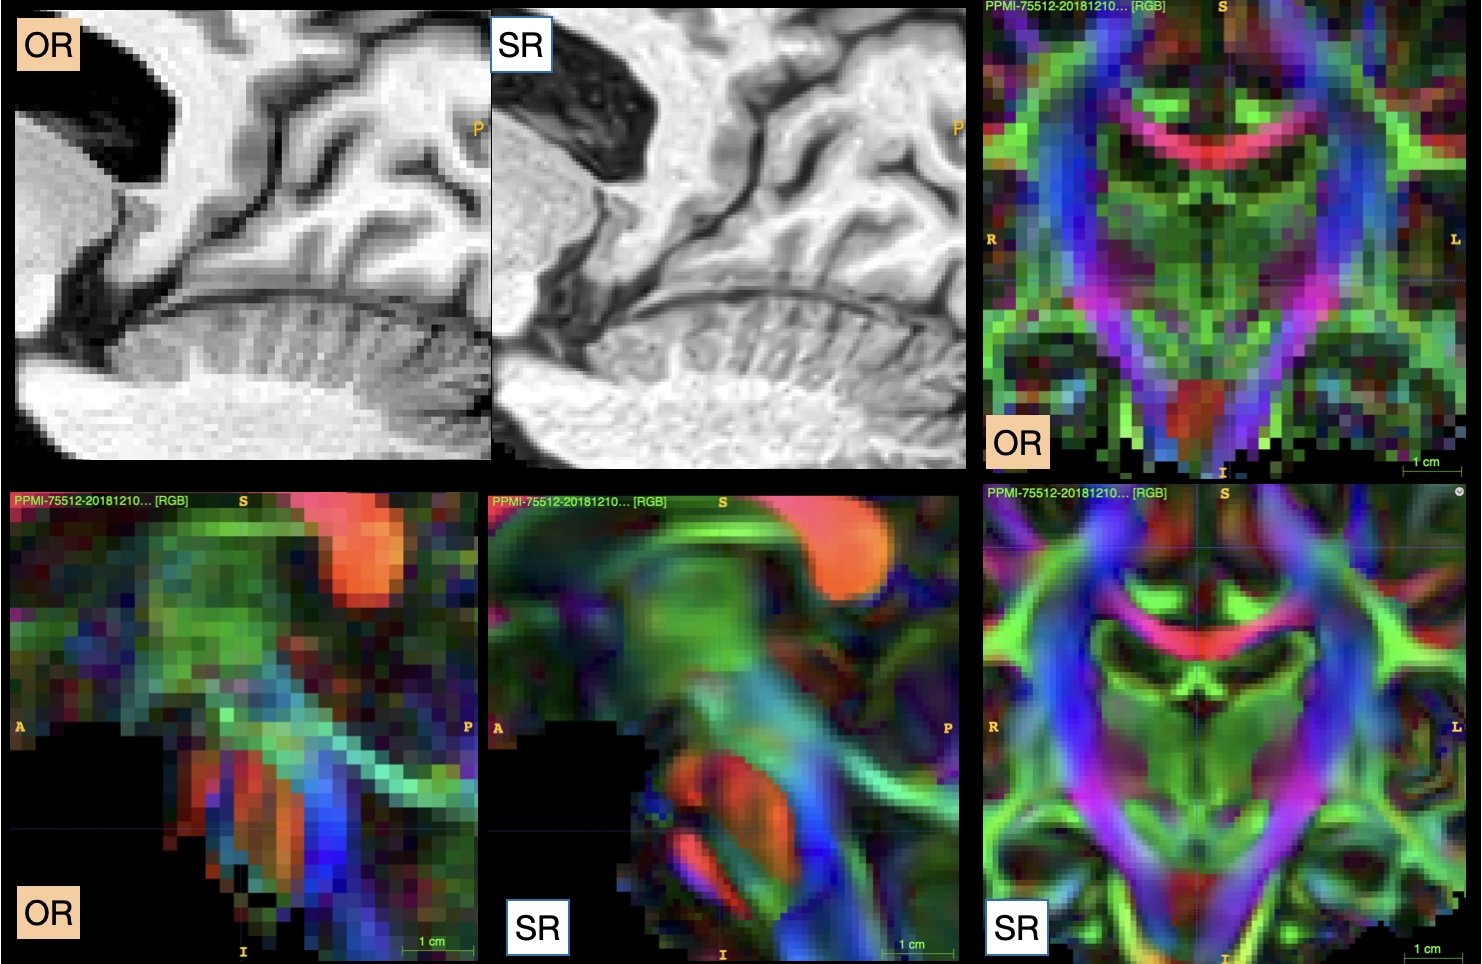
\includegraphics[keepaspectratio]{../figs/sr_comparison.jpg}}
\caption{Example ANTsPyMM SR outputs applied to sMRI (upper left) and
dMRI. T1w is super resolved to 0.5mm isotropic and dMRI to 1mm.}
\end{figure}

\subsubsection{Diffusion MRI processing}\label{diffusion-mri-processing}

Diffusion MRI processing to produce diffusion tensor images (DTI)
leverages best practices from both ANTsX
(\citeproc{ref-avants_pediatric_2015}{B. B. Avants et al. 2015};
\citeproc{ref-stone_neurological_2023}{Stone et al. 2023},
\citeproc{ref-stone_functional_2020}{2020}) and the open-source
dMRI-focused project \href{https://dipy.org}{DiPy}
(\citeproc{ref-garyfallidis_dipy_2014}{Garyfallidis et al. 2014}). This
pipeline is specifically designed to utilize dMRI acquisitions with
either a single or opposed phase encoding directions. The functionality
has been developed to address a broad spectrum of preprocessing
requirements, such as motion correction, denoising, dewarping and
gradient reorientation, and enhancement through SR techniques,
culminating in an optimized DTI reconstruction. The SR stream applies to
each volume in the dMRI timeseries after motion correction and
distortion correction but before tensor fitting i.e.~in a relatively
minimally invasive fashion. After reconstruction, the pipeline
integrates atlas-based labeling and template-based normalization
processes, thereby enhancing the anatomical interpretability of the DTI
metrics. Figure 4 summarizes the pipeline which follows these steps:

\begin{figure}
\centering
\pandocbounded{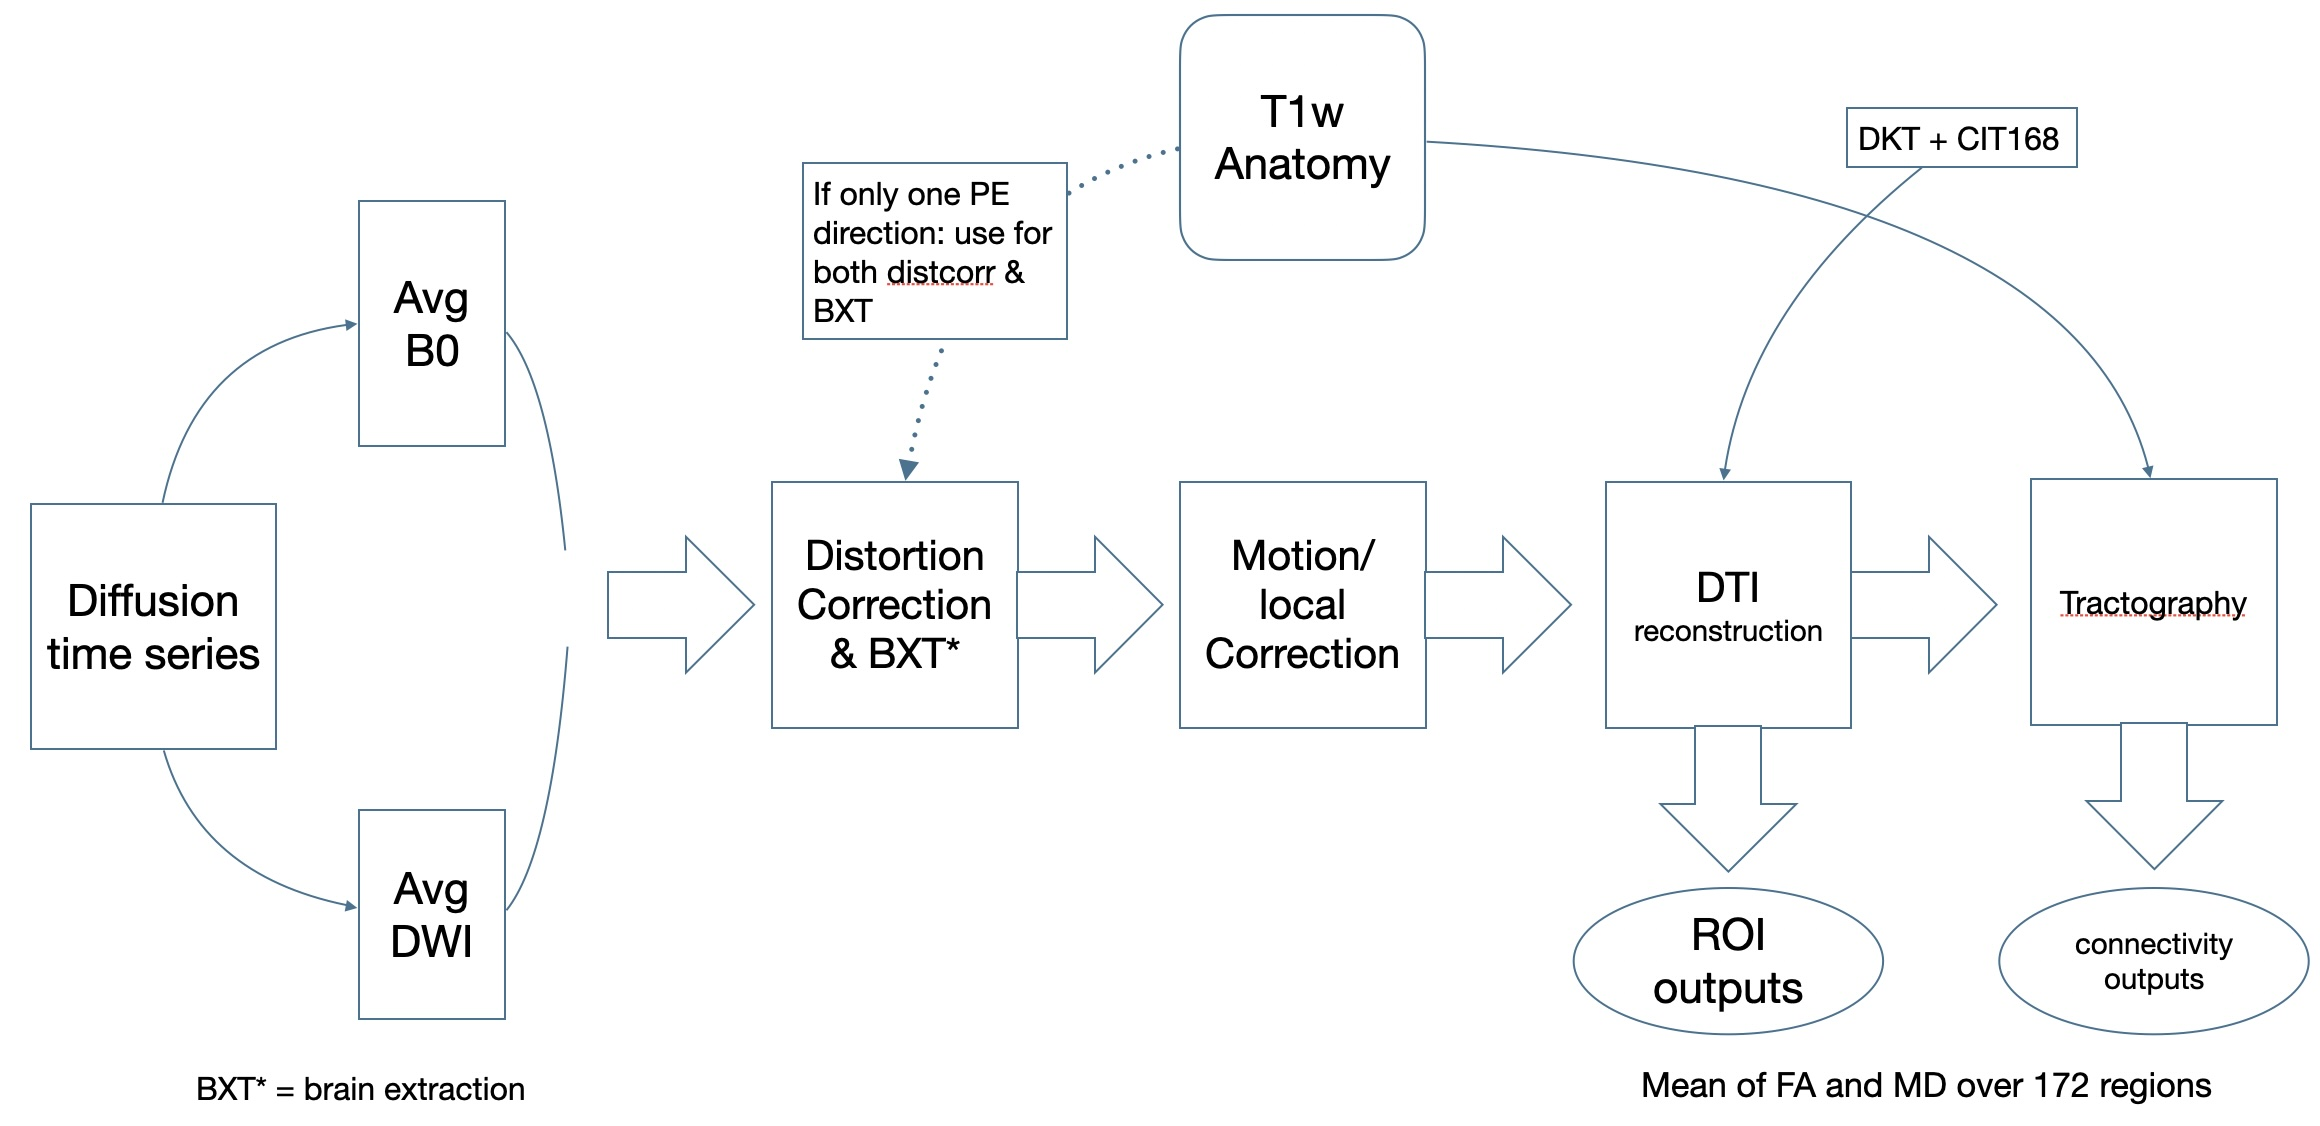
\includegraphics[keepaspectratio]{../figs/dti_pipe.jpg}}
\caption{Overview of the dMRI processing pipeline based on ANTsX and
DiPy.}
\end{figure}

\begin{enumerate}
\def\labelenumi{\arabic{enumi}.}
\item
  \textbf{Input Preparation}: The pipeline accepts either a single dMRI
  or a pair of dMRI with reversed phase encoding. It also requires
  associated b-values and b-vectors for each direction, alongside a
  T1-weighted image and a brain mask for improved spatial accuracy in
  inter-modality registration.
\item
  \textbf{Initial Reconstruction and Motion Correction}: By default, the
  dMRI data is denoised before performing motion correction. This is
  skipped when applying SR which integrates denoising. Motion correction
  aligns dMRI volumes within and across acquisitions to a reference mean
  B0 and mean dMRI, reducing artifacts due to subject movement.
\item
  \textbf{Dewarping and Super-Resolution}: Dewarping is applied to
  correct for distortions between the dMRI space and the T1-weighted
  image. Optionally, SR is applied after dewarping but before the DiPy
  based reconstruction process.
\item
  \textbf{Reconstruction of DTI Metrics}: The function employs weighted
  least squares to reconstruct DTI metrics such as Fractional Anisotropy
  (FA) and Mean Diffusivity (MD) from the preprocessed dMRI data. This
  step is pivotal in quantifying the diffusion properties of brain
  tissue.
\item
  \textbf{Atlas-Based Labeling and Registration}: Utilizing the Johns
  Hopkins University (JHU) atlas and corresponding labels
  (\citeproc{ref-mori_white_2009}{Mori, Oishi, and Faria 2009}), the
  pipeline performs spatial registration of the DTI to the atlas space.
  This process facilitates anatomical localization and quantification of
  DTI metrics within predefined brain regions.
\item
  \textbf{Output Generation}: The pipeline yields the reconstructed DTI
  metrics, summary statistics of these metrics within atlas-defined
  regions, the spatial registration information, and additional
  diagnostic metrics such as framewise displacement and signal-to-noise
  ratio (SNR) assessments spatially and temporally for both B0 and dMRI.
  An example output volumetric tensor image with labels is in Figure 3
  and 5.
\end{enumerate}

IDPs derived from the dMRI processing are denoted by prefixes
\texttt{DTI\_}.

\begin{figure}
\centering
\pandocbounded{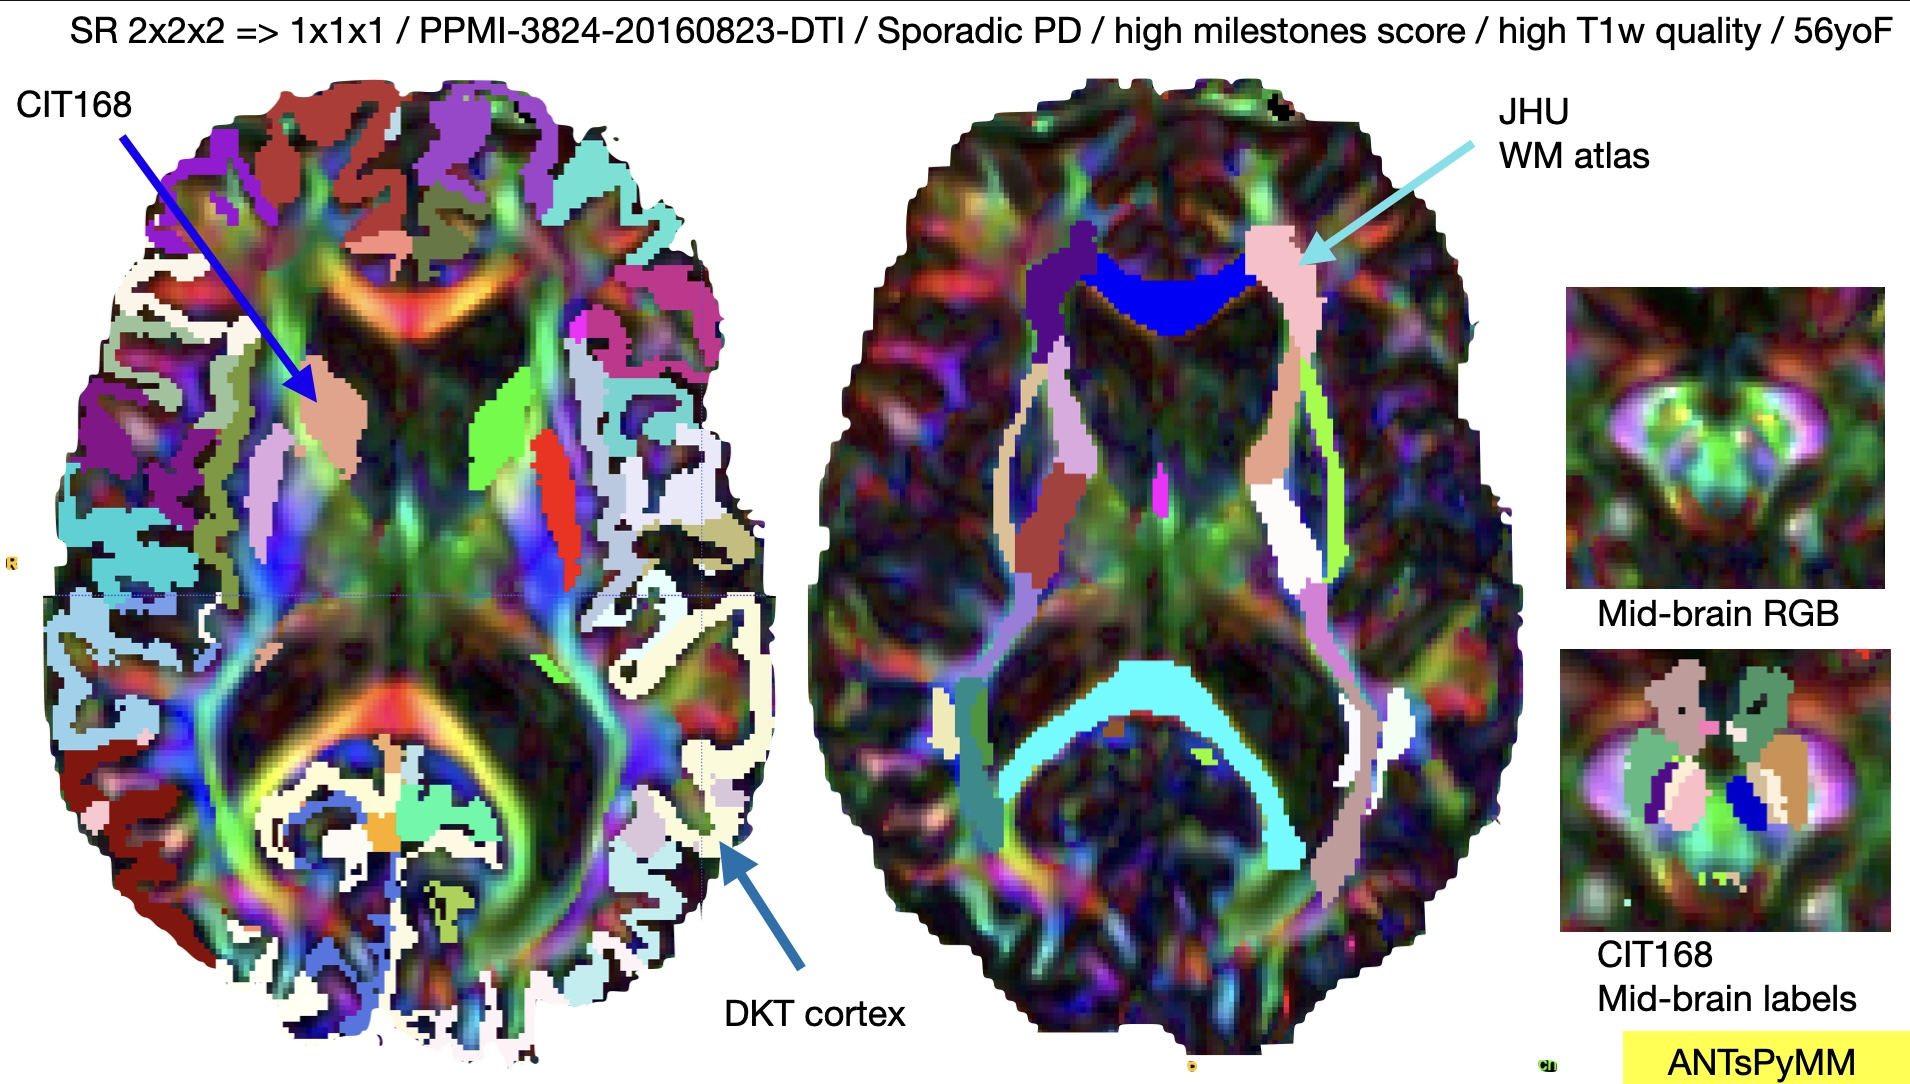
\includegraphics[keepaspectratio]{../figs/dti_SR.jpg}}
\caption{Example SR processing for dMRI highlighting the multiple
anatomical coordinate systems that aid interpretation.}
\end{figure}

\subsubsection{Resting state functional MRI
processing}\label{resting-state-functional-mri-processing}

Resting state functional MRI (rsfMRI) processing builds on prior
multi-view M3RI analyses performed in this same ecosystem
(\citeproc{ref-avants_pediatric_2015}{B. B. Avants et al. 2015},
\citeproc{ref-avants_amyloid_2019}{2019};
\citeproc{ref-avants_similarity-driven_2021}{B. B. Avants, Tustison, and
Stone 2021}). The procedure is based on the findings described in three
comprehensive evaluation studies
(\citeproc{ref-shirer_optimization_2015}{Shirer et al. 2015};
\citeproc{ref-parkes_evaluation_2018}{Parkes et al. 2018};
\citeproc{ref-noble_decade_2019}{Noble, Scheinost, and Constable 2019})
and is designed to compute both functional activity and correlation maps
utilizing the recently proposed homotopic labels to delineate major
network systems (\citeproc{ref-yan_homotopic_2023}{Yan et al. 2023}).
The methodology described below is grounded in contemporary
understanding of resting-state fMRI analysis and incorporates
recommendations from seminal works regarding optimal preprocessing for
minimizing motion artifacts and other sources of noise
(\citeproc{ref-shirer_optimization_2015}{Shirer et al. 2015};
\citeproc{ref-parkes_evaluation_2018}{Parkes et al. 2018}). As such, our
processing reflects an approach optimized for rsfMRI IDP extraction for
real-world multi-site studies of neurodegenerative disease. Overall, the
methods aim to facilitate the reliable extraction of functional
connectivity patterns that are consistent with underlying neural
mechanisms in PD (\citeproc{ref-tahmasian_systematic_2015}{Tahmasian et
al. 2015}; \citeproc{ref-esposito_rhythm-specific_2013}{Esposito et al.
2013}). Similar to the dMRI processing, the procedure accepts either a
single image or a pair of images with reversed phase encoding direction.
The steps are outlined in Figure 6:

\begin{figure}
\centering
\pandocbounded{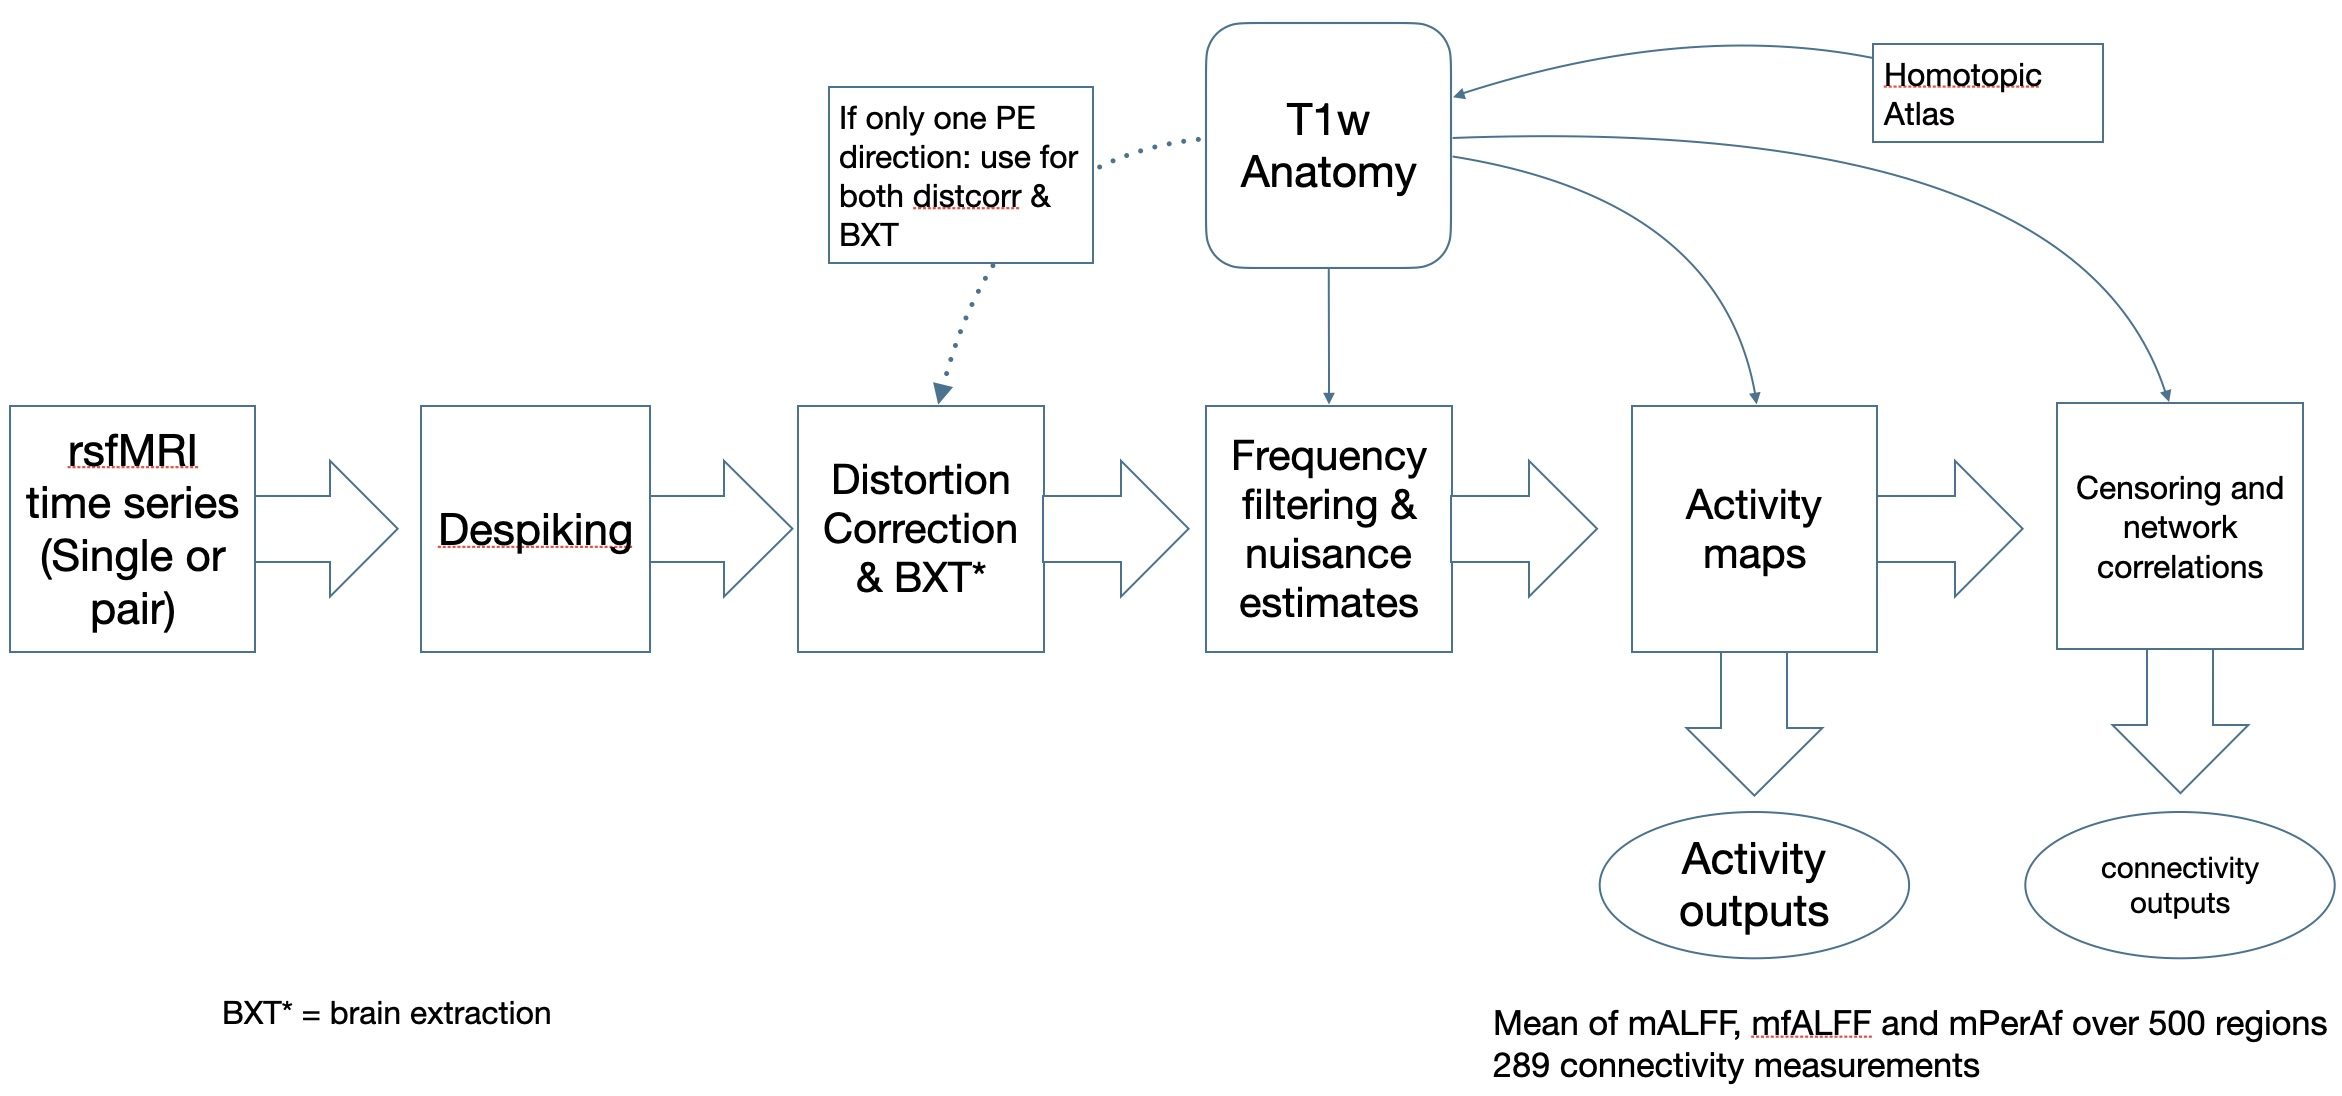
\includegraphics[keepaspectratio]{../figs/fmri_pipe.jpg}}
\caption{Overview of the rsfMRI processing pipeline based on ANTsX.}
\end{figure}

\begin{enumerate}
\def\labelenumi{\arabic{enumi}.}
\item
  \textbf{Input Preparation}: Inputs include the raw BOLD rsfMRI
  time-series data, a reference volumetric subject-specific rsfMRI
  template (automatically generated), and T1-weighted anatomical images
  all from the same subject. These inputs are foundational for aligning
  functional data with anatomical landmarks and for ensuring that
  subsequent analyses are anatomically informed. By default, the input
  rsfMRI is upsampled to 3mm isotropic resolution and 8 initial volumes
  are discarded to allow for both signal and subject stabilization.
\item
  \textbf{Preprocessing}: Initial steps include motion correction,
  application of a despiking algorithm (a \texttt{Python} implementation
  of AFNI's 3dDespike (\citeproc{ref-cox_afni_2012}{Cox 2012})), and
  anatomical registration to align the rsfMRI data with the T1-weighted
  image. If a pair of images is passed, these same preprocessing steps
  are applied and results are concatenated along the time axis.
\item
  \textbf{Noise Reduction}: Anatomical CompCor (aCompCor) is used to
  mitigate physiological and other noise sources. This is based on
  recommendations from studies examining the impact of preprocessing
  strategies on functional connectivity
  (\citeproc{ref-shirer_optimization_2015}{Shirer et al. 2015};
  \citeproc{ref-parkes_evaluation_2018}{Parkes et al. 2018}).
\item
  \textbf{Band-pass Filtering and activity calculation}: The application
  of a specific frequency range for filtering aligns with
  recommendations from both Shirer et al.~(2015) and Parkes et
  al.~(2018), emphasizing the importance of selecting appropriate
  frequency bands for resting-state analysis. The default frequency
  bands are based on empirical evaluation studies described below.
\item
  \textbf{Censoring}: Select volumes are censored based on both
  motion-based and intensity-based outlier detection. The parameters for
  this stage derive from empirical evaluation studies on public data as
  discussed below. Both \emph{censored} and \emph{imputed} versions of
  the time series are created. A summary of censoring results is
  recorded in several ways but perhaps most relevant are the variables
  \texttt{*minutes\_original\_data} and
  \texttt{*minutes\_censored\_data} which provides the length in minutes
  of the original versus processed data.
\item
  \textbf{Network Correlation Analysis}: This step involves calculating
  correlation matrices for identified resting-state networks, utilizing
  labels described above. Both inter and intra-network correlation
  values are computed for each of the sub-networks provided by the
  homotopic parcellation.
\item
  \textbf{Functional activity}: is computed with three models: mfALFF,
  mALFF and mPerAf as described in (\citeproc{ref-jia_percent_2020}{Jia
  et al. 2020}). These are versions of fALFF, ALFF and PerAf where each
  is divided by the global mean in the brain. Summary values are
  averaged within each of 500 labels in the homotopic label set which
  facilitates left/right asymmetry and mean values which are critical to
  studying diseases with laterality effects.
\end{enumerate}

Due to the relatively diverse needs of researchers and the variety of
rsfMRI that is generally present in public data, we run the above
processing with three different sets of parameters. These sets are named
by their position in the parameter search data frame as
\href{https://github.com/ANTsX/ANTsPyMM/blob/0d987b7c56d2d24a4a24ccb71dbb93d51157ff05/antspymm/mm.py\#L6596-L6605}{122,
134 and 129}. They encode a triplet of choices for outlier rejection
(based on motion) and control of nuisance signal via aCompCor. These
three parameter choices led to rsfMRI IDPs that were the top performers
in terms of reliability and predictive power out of 78 that we tested
empirically. See
\href{https://github.com/stnava/antspymm_reproducibility}{this
repository} and the technical validation section for further details.
IDPs from the rsfMRI processing are denoted by prefixes
\texttt{rsfMRI\_fcnxpro122} for 122 and similarly for 129 and 134.

\subsection{Dimensionality reduction with
SiMLR}\label{dimensionality-reduction-with-simlr}

Statistical power in cohorts with diverse composition may be challenged
by the number of individual predictors (here, 1178). To address this, we
adopt similarity-driven multi-view linear reconstruction (SiMLR) for
dimensionality reduction and apply the default settings recommended in
prior work (\citeproc{ref-avants_similarity-driven_2021}{B. B. Avants,
Tustison, and Stone 2021}; \citeproc{ref-stone_neurological_2023}{Stone
et al. 2023}). SiMLR provides a reduced number of predictors by creating
``sparse feature sets'' that are linked across modalities, allowing for
their combined use in joint prediction models. As an unsupervised
method, SiMLR identifies a joint low-dimensional space that captures the
common variability across these diverse modalities. This enables
integrated analyses of MRI and acquired non-imaging data (represented as
standard tabular outcomes) within the analytical framework of classical
regression. Importantly, this approach can be applied even when only a
subset of the variables is present.

Here, the SiMLR decomposition is trained in ADNI subjects and
subsequently applied to PPMI thereby decoupling the learning and
inference stages. Six matrices were decomposed into 100 joint
components. The matrices included one for tabular clinical data and five
for neuroimaging including T1w related measurements averaged across left
and right, T1w related asymmetry measurements, DTI related measurements
averaged across left and right, DTI related asymmetry measurements and
resting state connectivity measurements. Although cognition and
functionally related clinical scores were employed during decomposition,
these were not retained for further application to PPMI. The technical
validation section will demonstrate how these learned patterns may be
used in analyses integrating PPMI IDPs and clinically relevant metrics
both cross-sectionally and longitudinally.

\section{Data Records}\label{data-records}

The PPMI IDPs for sMRI, dMRI and rsfMRI are located at
(\citeproc{ref-avants_ppmi_2024}{B. Avants 2024}). The neuroimaging and
associated standard PPMI demographics and clinical data is hosted in the
\href{http://ida.loni.usc.edu}{LONI Imaging Data Archive (LONI IDA)}.
The former is stored in DICOM format and the latter in tabular
\texttt{csv} format. Additionally, data dictionaries describing all
non-imaging column headers are available on the LONI IDA.

We attach the neuroimaging IDPs to the PPMI Curated Data Cut
(v.2024-01-29 \texttt{PPMI\_Curated\_Data\_Cut\_Public\_20240129}) from
the LONI IDA. Code for this merging process is within the
\href{https://stnava.github.io/subtyper/}{subtyper package} specifically
the function
\href{https://stnava.github.io/subtyper/reference/merge_ppmi_imaging_clinical_demographic_data.html}{merge\_ppmi\_imaging\_clinical\_demographic\_data}.
The M3RI IDPs are described in detail
\href{http://htmlpreview.github.io/?https://github.com/stnava/ANTsPyMM/blob/main/docs/make_dict_table.html}{here}
and are in a data table within the \texttt{ANTsPyMM} repository (csv
format). The full tabular IDPs for both OR and SR outputs are at
\href{https://figshare.com/articles/dataset/PPMI_MR_IDPs/25361071}{this
location}.

We supplement these PPMI data with subjects from ADNI due to the current
dearth of control longitudinal neuroimaging in PPMI. As with PPMI, we
attach ANTsPyMM IDPs to \texttt{ADNIMERGE\_10Feb2024} using the
\texttt{subtyper} function
\texttt{merge\_ADNI\_antspymm\_by\_closest\_date}. Select subjects from
ADNI are considered for merging with PPMI if they are not diagnosed wtih
Alzheimer's disease or mild cognitive impairment (MCI) and have
acceptable quality neuroimaging. The ADNI cohort is significantly older
(mean of 72.3 years versus 63.9 in PPMI).

We also train a regression model on the matched subjects to adjust
imaging variables for systematic differences dut to study populations
(ADNI vs PPMI), MRI manufacturers (`GE', `Philips', `Siemens') and
magnetic field strength. Control subjects aged between 50 and 70 are
designated as training samples. The regression map is learned and
applied to each IDP throughout the full cohort using the
\texttt{subtyper} function \texttt{adjustByCovariates}. The purpose of
this process is to mitigate the influence of different imaging
protocols, ensuring that subsequent analyses are less confounded by
these factors. This approach has been used in practical studies of ADNI
MRI data (\citeproc{ref-Risacher2017}{Risacher et al. 2017}). These
merged and adjusted IDP data records are included in the file
\texttt{ppmi\_idps\_trim\_v1.4.0\_SRF.csv}. SiMLR derived variables are
denoted \texttt{t1PC*} (left-right averaged T1w derived feature sets),
\texttt{t1aPC*} (asymmetry-related T1w derived feature sets),
\texttt{dtPC*} (left-right averaged DTI derived feature sets),
\texttt{dtaPC*} (asymmetry-related DTI derived feature sets) and
\texttt{rsfPC*} (resting connectivity) where the \texttt{*} varies from
1 to 100. These SiMLR derived variables limit the multiple testing
considerations to 100 variables because these are typically grouped
together. That is, a given PC set (referred to as \(simIDP_i^k\)) is
included in a single model (e.g.~if \(k=1\), then
\(age \approx t1PC1 + t1aPC1 + dt1PC1 + dtaPC1 + rsfPC1\)) where
\(simIDP_1=t1, simIDP_2=t1a\), etc. We use this approach in a technical
validation section below.

\section{Technical Validation}\label{technical-validation}

Components of technical validity that are critical for quantitative
methodology in neuroimaging include: (a) generally robust performance
across modalities; (b) multi-site reproducibility; (c) disease-specific
discrimination from controls in particular over time in the clinical
trial setting; (d) sensitivity to or relationship with changes in
clinically relevant symptoms at baseline and/or over time. We provide
evidence that the current IDPs satisfy these properties in the following
sections.

\begin{itemize}
\item
  We quantify reproducibility and reliability in each modality through
  analysis of three traveling subject cohorts (addressing (a) and (b)
  above). These cohorts collect imaging data at different sites from the
  same individuals. Reliability data based on such cohorts are highly
  relevant for multisite trials which are always impacted by
  site-specific variation. By aggregating data from the traveling
  subject cohorts, we offer precise, reproducible reliability estimates
  (via intra-class correlation) manifested across different scanner
  types and imaging modalities.
\item
  We derive effect sizes from statistical models that test established
  hypotheses comparing biomarker classified sporadic PD subjects versus
  control subjects. These show expected effects of PD are detectable in
  these data. This addresses (c) above.
\item
  We finalize the technical validity section with examples of how
  scientists may relate IDP measures of brain health to rate of symptom
  change in PD in a multiple modality (integrative) context. This
  addresses (d) above.
\end{itemize}

The scale of the current data supports control for a subset of important
PD relevant covariates including disease duration, educational level,
sex, age and levodopa dose equivalent daily dose (LEDD). These variables
are included in reference models with additional details below.

\subsection{Robust performance}\label{robust-performance}

The technical validity of these methods is supported by previous work,
including various open quantitative MRI analysis challenges
(\citeproc{ref-menze_multimodal_2015}{Menze et al. 2015};
\citeproc{ref-murphy_evaluation_2011}{Murphy et al. 2011};
\citeproc{ref-baheti_brain_2021}{Baheti et al. 2021}) that span
modalities and organ systems. The foundational methods also support
applications to non-human data
(\citeproc{ref-allan_johnson_whole_2019}{Allan Johnson et al. 2019};
\citeproc{ref-hopkins_regional_2013-1}{Hopkins and Avants 2013}).
Furthermore, the consistency of the methodology naturally enables
multivariate statistical inference and/or prediction
(\citeproc{ref-stone_neurological_2023}{Stone et al. 2023}) even within
the multi-study context (\citeproc{ref-dadu_prediction_2024}{Dadu et al.
2024}).

\subsection{Multi-site
reproducibility}\label{multi-site-reproducibility}

Traveling subject studies involve scanning the same subjects on multiple
MRI scanners at different locations. These studies help in assessing
consistency and/or agreement of image quantification where the only
variables are the machines themselves. This is crucial for understanding
power in multi-site studies of natural history or intervention and for
ensuring that the observed changes in brain structure or function are
due to actual physiological changes rather than variations in the
imaging process itself.

In this study, we employ traveling cohort data
(\citeproc{ref-hawco_longitudinal_2022}{Hawco et al. 2022};
\citeproc{ref-tanaka_multi-site_2021}{Tanaka et al. 2021};
\citeproc{ref-tong_reproducibility_2019}{Tong et al. 2019}) to assess
the agreement of IDPs pooled across multiple sites for the purposes of
statistical inference. These data will establish expectations of
repeatability for sMRI, dMRI and rsfMRI as measured by ANTsPyMM
processing and are described briefly here:

\begin{enumerate}
\def\labelenumi{\arabic{enumi}.}
\tightlist
\item
  the SRPBS Traveling Subject MRI Dataset
  (\citeproc{ref-tanaka_multi-site_2021}{Tanaka et al. 2021}):
\end{enumerate}

\begin{itemize}
\item
  9 healthy subjects travel to 12 sites to be imaged;
\item
  of the 12 sites, 9 have consistently available sMRI and rsfMRI in 6
  subjects.
\end{itemize}

\begin{enumerate}
\def\labelenumi{\arabic{enumi}.}
\setcounter{enumi}{1}
\tightlist
\item
  traveling subject dMRI cohort
  (\citeproc{ref-tong_reproducibility_2019}{Tong et al. 2019}):
\end{enumerate}

\begin{itemize}
\item
  3 healthy subjects travel to 4 sites to be imaged;
\item
  T1w and multi-shell dMRI are available.
\end{itemize}

\begin{enumerate}
\def\labelenumi{\arabic{enumi}.}
\setcounter{enumi}{2}
\tightlist
\item
  Hawco's traveling subject MRI dataset
  (\citeproc{ref-hawco_longitudinal_2022}{Hawco et al. 2022}) is
  available \href{https://openneuro.org/datasets/ds003011}{here}:
\end{enumerate}

\begin{itemize}
\tightlist
\item
  4 healthy male subjects travel to 6 sites to be imaged with T1w,
  rsfMRI and dMRI.
\end{itemize}

Thus, we use these data to characterize the consistency and reliability
of these tools when applied to data that has known systematic biases due
to site and scanner differences. The results confirm that findings and
conclusions drawn from ANTsPyMM are reliable and not overwhelmed by
scanner-specific differences or inconsistencies. This knowledge is
critical for a foundational framework such as ANTsX/ANTsPyMM upon which
scientific studies, machine learning platforms and other methodological
comparisons are based. These cohorts represent variability in both MRI
manufacturer and MRI model (high variability) that would exceed standard
(within-scanner, within-site) test-retest analysis. Results therefore
provide a lower-bound on reliability; i.e.~within-site
(e.g.~longitudinal) studies would be expected to have higher reliability
in general.

\begin{figure}
\centering
\pandocbounded{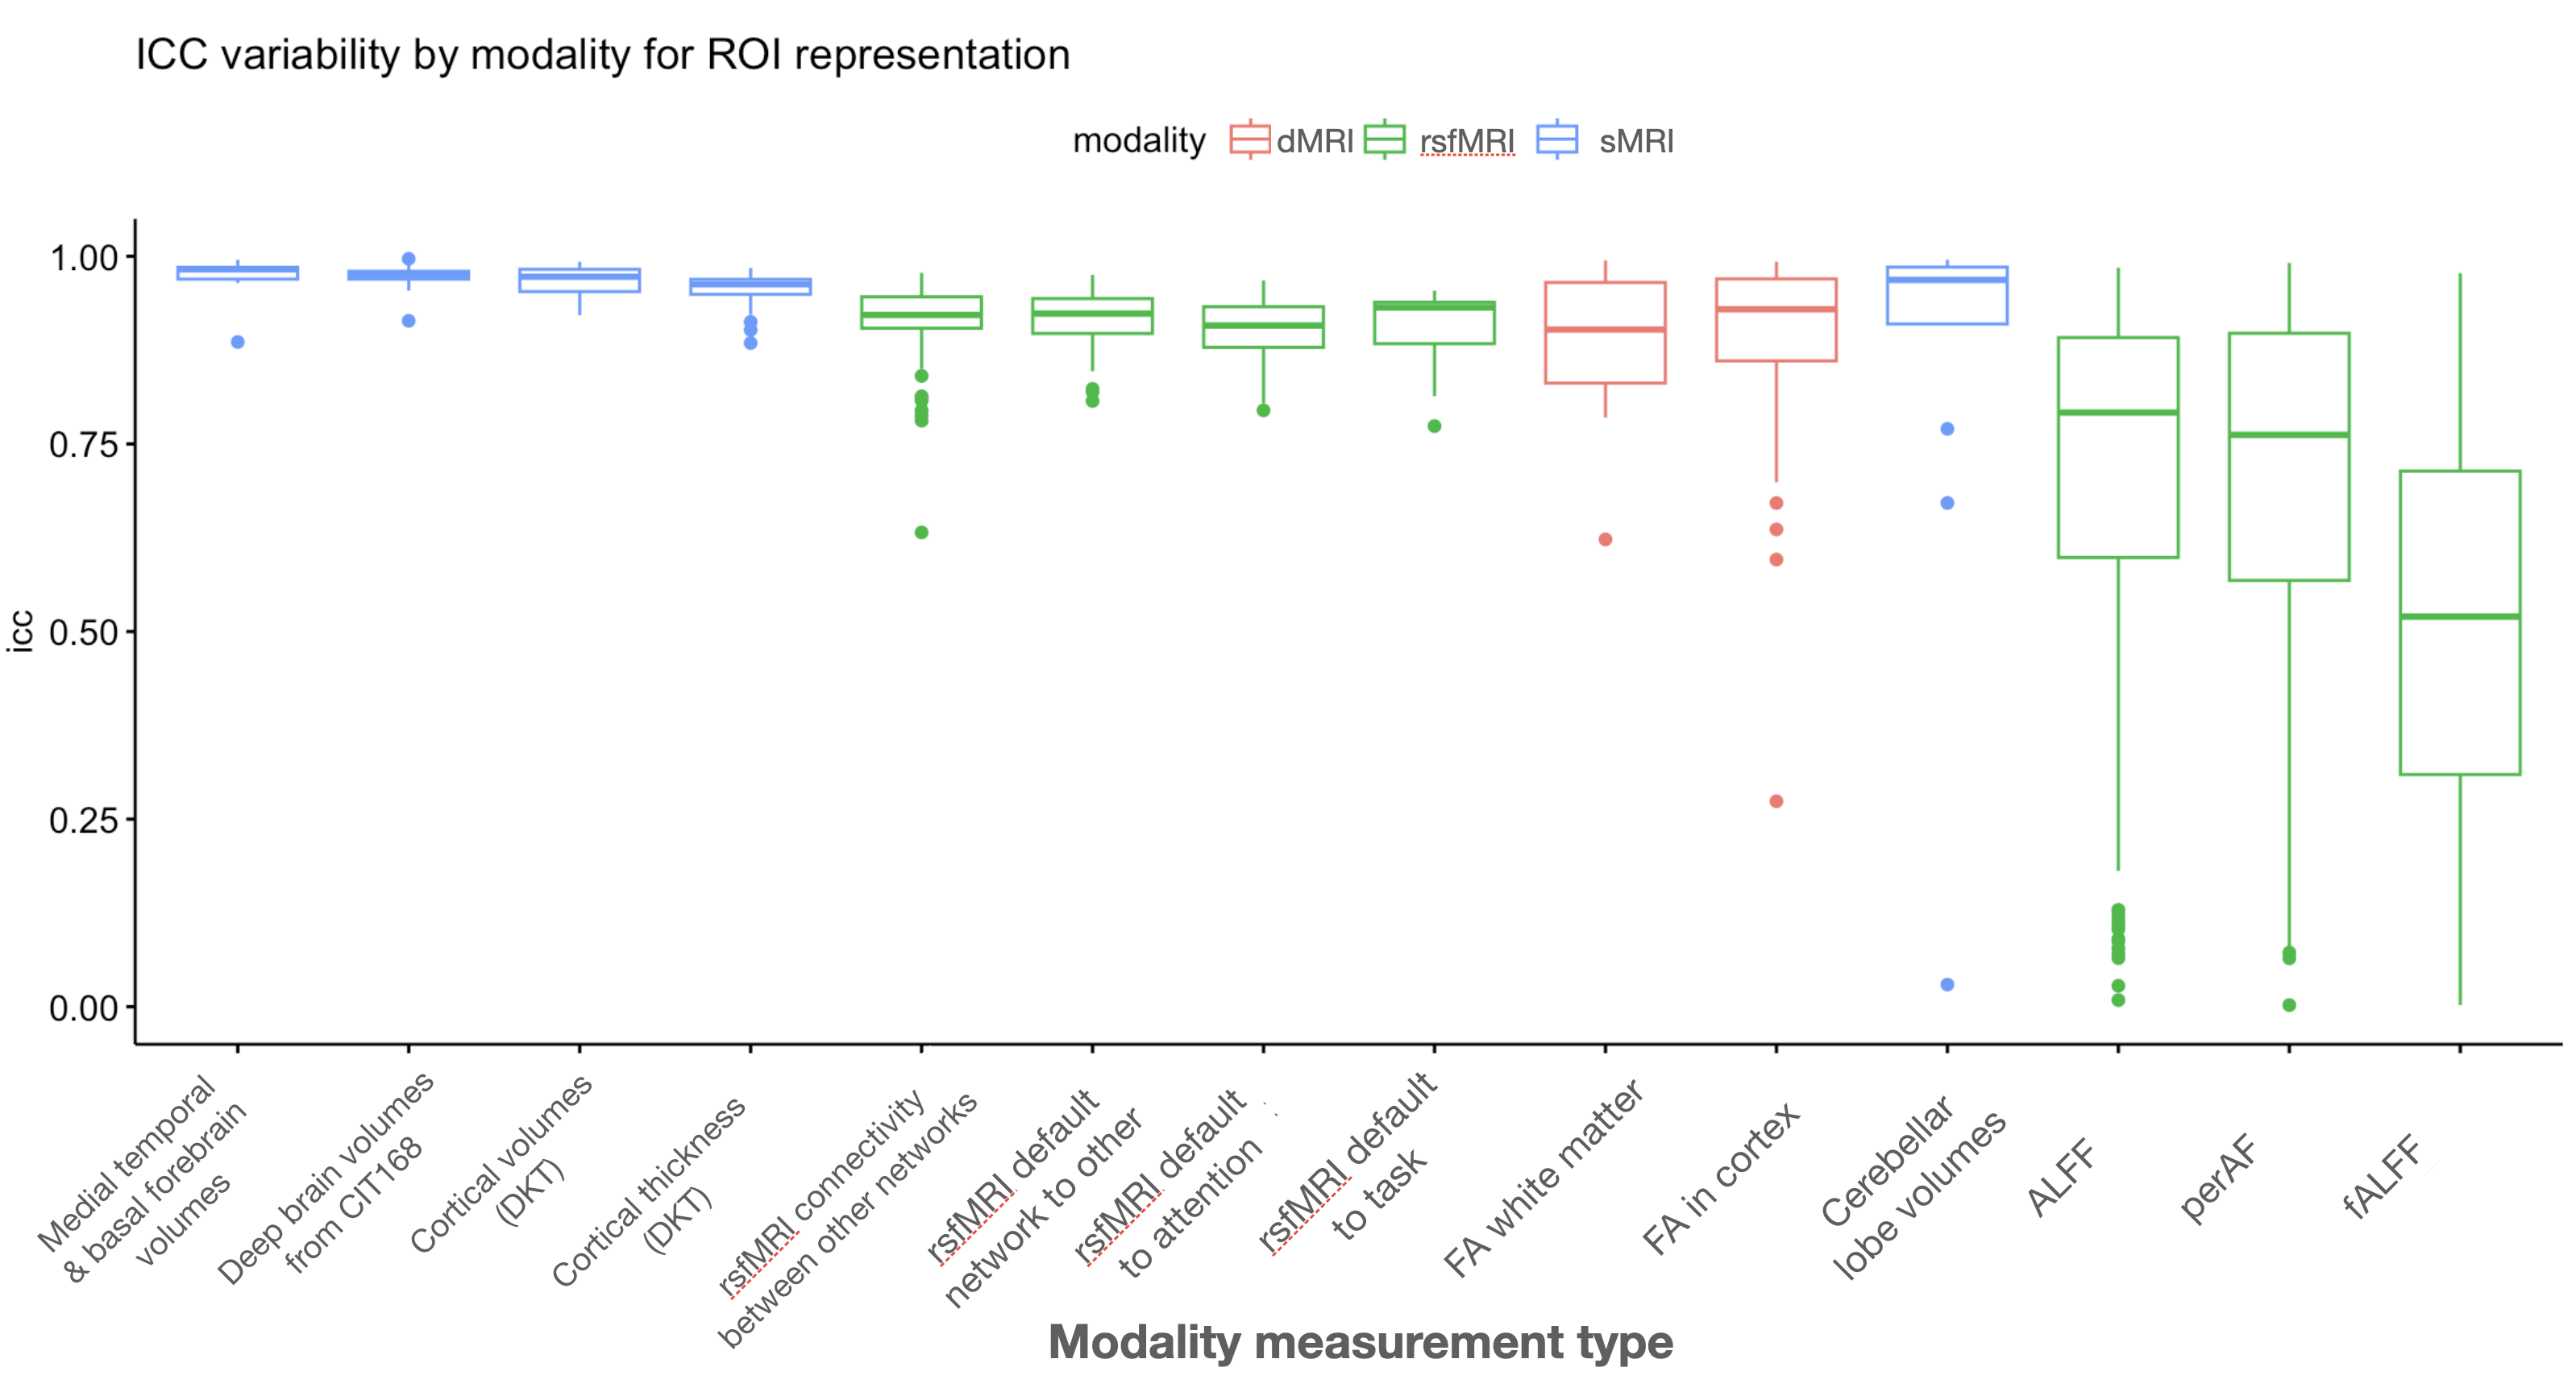
\includegraphics[keepaspectratio]{../figs/antspymm_repro.png}}
\caption{Summary reproducibility results from aggregated traveling
subject data. sMRI (T1w) IDPs represent high reproducibility in all
categories (cerebellum, CIT168, cortical volume, cortical thickness,
basal forebrain and medial temporal lobe). dMRI IDPs are also highly
reproducible with FA in the cortical gray matter (gm) nearly equaling
that of major white matter regions in the JHU atlas. Resting state
connectivity shows good to excellent reproducibility; PerAF, fALFF and
ALFF are relatively less reproducible -- on average -- though
variability across regions is also high.}
\end{figure}

We employ the intra-class correlation to assess results. ICC ranges may
be interpreted as (\citeproc{ref-koo_guideline_2016}{Koo and Li 2016}):

\begin{itemize}
\item
  below 0.50: poor
\item
  between 0.50 and 0.75: moderate
\item
  between 0.75 and 0.90: good
\item
  above 0.90: excellent
\end{itemize}

We find that ANTsPyMM IDPs derived from the same subjects imaged at
different sites with MRI from various manufacturers show overall good to
high reliability with a few exceptions within resting state derivatives
(fALFF specifically). This provides empirical evidence that multiple
modality MRI may be used to derive quantitative phenotypes on which
predictive models may be based. Statistical control for site effects
should still be applied at the population level using, for example,
random effects. The data and code for reproducing these results is
available in
\href{https://github.com/stnava/antspymm_reproducibility}{this
location}. Figure 7 shows the key summary output for this ICC
comparison.

\definecolor{platinum}{rgb}{0.9, 0.89, 0.89} 
\definecolor{black}{rgb}{0.0, 0.0, 0.0} 
\begin{small}
\color{black}
\begin{tabular}{ll}
\multicolumn{2}{c}{Table 3. PD IDPs in ANTsPyMM: T1w L/R average and asym.}\\ 
\hline
\textbf{IDP}&\textbf{anat}\\ 
\hline
\cellcolor{platinum}t1.vol.sup.parietal.ctx&\cellcolor{platinum}Superior Parietal Cortex\\ 
t1.vol.inf.parietal.ctx&Inferior Parietal Cortex\\ 
\cellcolor{platinum}t1.vol.paracent.ctx&\cellcolor{platinum}Paracentral Cortex\\ 
t1.vol.postcent.ctx&Postcentral Cortex\\ 
\cellcolor{platinum}t1.vol.precent.ctx&\cellcolor{platinum}Precentral Cortex\\ 
t1.vol.sncdp.&Substantia Nigra Compacta\\ 
\cellcolor{platinum}t1.vol.bn.str.pudp.&\cellcolor{platinum}Basal Nucleus Striatum, Putamen\\ 
t1.vol.bn.gp.gpidp.&Globus Pallidus Internal Segment\\ 
\cellcolor{platinum}t1.vol.bn.gp.gpedp.&\cellcolor{platinum}Globus Pallidus External Segment\\ 
t1.vol.nbm.antbf&Nucleus Basalis Meynert, Anterior Basal Forebrain\\ 
\cellcolor{platinum}t1.vol.nbm.midbf&\cellcolor{platinum}Nucleus Basalis Meynert, Middle Basal Forebrain\\ 
t1.vol.nbm.posbf&Nucleus Basalis Meynert, Posterior Basal Forebrain\\ 
\cellcolor{platinum}t1.vol.dg.ca3mtl&\cellcolor{platinum}Dentate Gyrus, CA3 Region of Medial Temporal Lobe\\ 
t1.midbrain.pons.ratio&Midbrain Pons ratio\\ 
\hline
\end{tabular}
\end{small}
\color{black}

\definecolor{platinum}{rgb}{0.9, 0.89, 0.89} 
\definecolor{black}{rgb}{0.0, 0.0, 0.0} 
\begin{small}
\color{black}
\begin{tabular}{ll}
\multicolumn{2}{c}{\begin{minipage}[c]{0.8\linewidth}Table 4. PD IDPs in ANTsPyMM: DTI L/R average and asym for both fractional anisotropy (FA) and mean diffusion (MD) (not shown).\end{minipage}}\\ 
\hline
\textbf{IDP}&\textbf{anat}\\ 
\hline
\cellcolor{platinum}dti.fa.sup.l.fasc&\cellcolor{platinum}Superior Longitudinal Fasciculus FA\\ 
dti.fa.deep.snc&Deep Substantia Nigra Compacta FA\\ 
\cellcolor{platinum}dti.fa.snc&\cellcolor{platinum}Substantia Nigra Compacta FA\\ 
dti.fa.sup.cor.rad&Superior Corona Radiata FA\\ 
\cellcolor{platinum}dti.fa.fornixlravg&\cellcolor{platinum}Fornix FA\\ 
dti.fa.ant.int.cap&Anterior Internal Capsule FA\\ 
\cellcolor{platinum}dti.fa.ext.cap&\cellcolor{platinum}External Capsule FA\\ 
dti.fa.post.int.cap&Posterior Internal Capsule FA\\ 
\cellcolor{platinum}dti.fa.rent.int.cap.&\cellcolor{platinum}Retrolenticular Part of Internal Capsule FA\\ 
dti.fa.sup.frnt.occ.fasc&Superior Frontal-Occipital Fasciculus FA\\ 
\cellcolor{platinum}dti.fa.deep.bn.str.pu&\cellcolor{platinum}Deep Basal Nucleus Striatum, Putamen FA\\ 
dti.fa.bn.str.pu&Basal Nucleus Striatum, Putamen FA\\ 
\hline
\end{tabular}
\end{small}
\color{black}

\definecolor{platinum}{rgb}{0.9, 0.89, 0.89} 
\definecolor{black}{rgb}{0.0, 0.0, 0.0} 
\begin{small}
\color{black}
\begin{tabular}{ll}
\multicolumn{2}{c}{\begin{minipage}[c]{0.670588235294118\linewidth}Table 5. PD IDPs in ANTsPyMM: rsfMRI bilateral inter or intra-network connectivity  (Yan, et. al. homotopic parcellation nomenclature).\end{minipage}}\\ 
\hline
\textbf{IDP}&\textbf{connectivity}\\ 
\hline
\cellcolor{platinum}rsf.p2.sommotb.2.temppar&\cellcolor{platinum}Temporal Parietal Region\\ 
rsf.p2.sommotb.2.contc&Control Network Component C\\ 
\cellcolor{platinum}rsf.p2.sommotb.2.contb&\cellcolor{platinum}Control Network Component B\\ 
rsf.p2.sommotb.2.conta&Control Network Component A\\ 
\cellcolor{platinum}rsf.p2.sommotb.2.sommotb&\cellcolor{platinum}Somatomotor Area B\\ 
rsf.p2.sommotb.2.sommota&Somatomotor Area A\\ 
\cellcolor{platinum}rsf.p2.sommotb.2.visperi&\cellcolor{platinum}Peripheral Visual Area\\ 
rsf.p2.sommotb.2.viscent&Central Visual Area\\ 
\cellcolor{platinum}rsf.p2.sommotb.2.striatum&\cellcolor{platinum}Striatum\\ 
rsf.p2.sommotb.2.dopamine&Dopaminergic system\\ 
\cellcolor{platinum}rsf.p2.sommotb.2.basalganglia&\cellcolor{platinum}Basal Ganglia\\ 
rsf.p2.sommotb.2.midbrain&Midbrain\\ 
\cellcolor{platinum}rsf.p2.sommota.2.temppar&\cellcolor{platinum}Temporal Parietal Region\\ 
rsf.p2.sommota.2.contc&Control Network Component C\\ 
\cellcolor{platinum}rsf.p2.sommota.2.contb&\cellcolor{platinum}Control Network Component B\\ 
rsf.p2.sommota.2.conta&Control Network Component A\\ 
\cellcolor{platinum}rsf.p2.sommota.2.sommotb&\cellcolor{platinum}Somatomotor Area B\\ 
rsf.p2.sommota.2.sommota&Somatomotor Area A\\ 
\cellcolor{platinum}rsf.p2.sommota.2.visperi&\cellcolor{platinum}Peripheral Visual Area\\ 
rsf.p2.sommota.2.viscent&Central Visual Area\\ 
\cellcolor{platinum}rsf.p2.sommota.2.striatum&\cellcolor{platinum}Striatum\\ 
rsf.p2.sommota.2.dopamine&Dopaminergic system\\ 
\cellcolor{platinum}rsf.p2.sommota.2.basalganglia&\cellcolor{platinum}Basal Ganglia\\ 
rsf.p2.sommota.2.midbrain&Midbrain\\ 
\hline
\end{tabular}
\end{small}
\color{black}

\begin{figure}
\centering
\pandocbounded{\includegraphics[keepaspectratio]{ppmi_sci_data_SRF_files/figure-latex/quicklmdxsetdown-1.pdf}}
\caption{Partial regression plots for example significant IDPs
illustrate the trends of differences from controls. The bar plots at
left show 95 percent confidence intervals along with estimated means for
each baseline group difference. The line plots at right show the
estimated change over time (zero to two years) along with 95 percent
confidence intervals. Table 6 and Table 7 detail the associated
significance levels and effect sizes.}
\end{figure}

\subsection{IDP differences in SAA+ and SAA- sporadic PD versus
controls}\label{idp-differences-in-saa-and-saa--sporadic-pd-versus-controls}

This section establishes reference models and associated effect sizes
comparing controls to SAA+ sporadic PD and SAA- sporadic PD subjects.
Symptoms of PD exhibit heterogeneity both across individuals and within
a single patient over time. MRI is suited to objective \emph{in vivo}
characterization of the neural basis of these changes longitudinally
with a variety of structural and functional measurements. Here, we
assess longitudinal and cross-sectional effect sizes within IDPs that
are pre-defined for PD relevance. These regions are listed in Table 3
(sMRI), Table 4 (dMRI) and Table 5 (rsfMRI) and span motor, associative
and limbic systems that may be impacted in PD and associated disorders
(\citeproc{ref-ryman_mri_2020}{Ryman and Poston 2020}). These include
motor and parietal cortex
(\citeproc{ref-filippi_progressive_2020}{Filippi et al. 2020};
\citeproc{ref-sokolowski_longitudinal_2024}{Sokołowski et al. 2024}),
midbrain and striatal regions and basal forebrain
(\citeproc{ref-batzu_increased_2023}{Batzu et al. 2023}) from T1w. Due
to known concomitant, AD-related pathology in some PD subjects, we also
include a medial temporal lobe IDP
(\citeproc{ref-das_episodic_2019}{Das, Hwang, and Poston 2019}).
Relatedly, we select mean diffusion and FA derived from DTI in the
striatum and substantia nigra (\citeproc{ref-hu_diffusion_2023}{Hu et
al. 2023}) as well as major white matter tracts
(\citeproc{ref-gattellaro_white_2009}{Gattellaro et al. 2009};
\citeproc{ref-pietracupa_freezing_2018}{Pietracupa et al. 2018}), the
fornix and external and internal capsule; a recent large-scale study
demonstrated sensitivity of these measures to PD
(\citeproc{ref-owens-walton_worldwide_2024}{Owens-Walton et al. 2024}).
Interestingly, DTI metrics in early PD -- within both the current study
and the recent worldwide study
(\citeproc{ref-owens-walton_worldwide_2024}{Owens-Walton et al. 2024})
-- appear to trend in directions that are opposite to that of other
neurodegenerative diseases which provides an opportunity for future work
and more nuanced stage-based statistical modeling. In rsfMRI, we focus
on connectivity between sensorimotor regions and other networks, in
particular visual and cognitive control
(\citeproc{ref-caspers_within_2021}{Caspers et al. 2021};
\citeproc{ref-wang_investigation_2021}{Wang et al. 2021};
\citeproc{ref-tahmasian_systematic_2015}{Tahmasian et al. 2015}). In
total, we test 99 different measurements which include left-right
averaged as well as asymmetry metrics: \[
avg(x_l,x_r)=\frac{1}{2}(x_l+x_r);~~~asym(x_l,x_r)=|x_l-x_r|
\] derived from those regions which are bilateral. This strategy is a
generalizable way of testing laterality effects across all groups,
including those without an established dominant side of disease
(controls and pre-symptomatic PD subjects).

We provide exemplar linear mixed-effects models (LMMs) that seek to
elucidate the complex relationships between neuroimaging biomarkers and
the progression of idiopathic PD. The analytical framework was
constructed using the \texttt{R} programming environment, leveraging the
\texttt{lme4} package
(\citeproc{ref-kuznetsova_lmertest_2017}{Kuznetsova, Brockhoff, and
Christensen 2017}; \citeproc{ref-bates_fitting_2014}{Bates et al.
2014}). This methodology allows for the exploration of hierarchical data
structures commonly encountered in longitudinal neuroimaging studies,
where multiple observations per subject are standard. These models were
designed to investigate differences between biomarker-confirmed sporadic
PD groups and controls. Here, we focus on SAA\(+\) and SAA\(-\) sporadic
PD groups. We accentuate that these models are for demonstration only
and do not constitute fully-vetted ``official'' PPMI results. While
these models may not account for all relevant covariates, they do
provide evidence of validity by confirming the sensitivity of these IDPs
to diagnostic group differences. These models are of the form:

\[
\begin{split}
\text{IDP } \approx (1|ID) + (1|Site) + \text{BV}_\text{bl} + Edu + duration_\text{yrs} + \\
  modality\_specific\_covariates  + age_\text{bl} + \\ 
  Sex_\text{bio}  + years_\text{bl}   *  \text{DX}
\end{split}
\]

where IDP is the imaging outcome, \(ID\) is a random effect for subject
ID, \(Site\) is a random effect for data collection site,
\(\text{BV}_\text{bl}\) is baseline brain volume, \(Edu\) is educational
attainment and \(modality\_specific\_covariates\) covaries for
modality-specific variability due to site and related effects. Age at
baseline and biological sex are additional covariates. The primary
predictors of interest are \(years_\text{bl}   *  \text{DX}\) i.e.~the
interaction between time from baseline of the IDP measurement (in years)
and the diagnostic group which includes SAA positive and negative
sporadic PD subjects in addition to controls. The
cross-sectional/longitudinal sample sizes and results for each group
within the \(DX\) variable are denoted in Table 6 (cross-sectional) and
Table 7(longitudinal) where a postfix of ``.x'' indicates a
cross-sectional estimate and ``.y'' a longitudinal one. The columns
\texttt{anv.x} and \texttt{anv.y} reflect omnibus model \(p\)-values;
\texttt{d} indicates effect size for the corresponding group either
cross-sectionally or longitudinally. The \texttt{sig} column indicates
whether the corrected \(p\)-value survives family-wise error (fwe) or
false discovery rate (fdr) correction. In the longitudinal cohort,
subjects are required to have two or more visits.

Cross-sectional models used standard linear regression (\texttt{lm} in
\texttt{R}) with the same structure as described above but without
random effects. Linear mixed-effects models (LMMs) were constructed
using the \texttt{lmer} function from the \texttt{lme4} package and
fitted to the data. This process included the standardization of
variables within the equation, a critical step given the varying scales
and distributions of neuroimaging metrics. Comparative model analysis
was conducted to ascertain the significance of various predictors,
employing the \texttt{anova} function to contrast models with and
without \(DX\) and the interaction between \(DX\) and
\(years_\text{bl}\). This \texttt{anova} assesses the ``omnibus'' model
improvement due to the joint addition of both \(DX\) and the interaction
between \(DX\) and \(years_\text{bl}\). As we are only reporting high
level results here, we do not investigate \(p\)-values within individual
diagnostic groups. These results are shown in Table 6 (for the \(DX\)
term) and Table 7 (for the longitudinal term). Effect sizes (d.x and
d.y) for each term are estimated from the \(t-\)value and degrees of
freedom for each cross-sectional and longitudinal model. Very small
effect sizes are those with absolute value less than 0.2. The effects of
\(DX\) on these IDPs are visualized through predictor effect plots
(\citeproc{ref-larsen_use_1972}{Larsen and McCleary 1972};
\citeproc{ref-JSSv087i09}{Fox and Weisberg 2018}) of diagnosis by time
generated for each diagnostic category as in Figure 8. These IDPs are
significant under family wise error (fwe) multiple comparisons
correction at \(p\)-value \(\le\) 0.05 (after correction based on the
above-mentioned \texttt{anova}). These plots and other regression plots
are displayed with the \texttt{R} packages
\href{https://jtools.jacob-long.com}{\texttt{jtools}} and
\href{https://interactions.jacob-long.com}{\texttt{interactions}}.

\setcounter{table}{5} \renewcommand{\thetable}{\arabic{table}}

\begin{landscape}\begin{table}

\caption{\label{tab:dxresults}Baseline group effects: SAA+/- sporadic PD vs. controls. n.x = sample size; anv.x = anova-based p value. d.x indicates effect size. sig indicates the level of significance.}
\centering
\begin{tabular}[t]{lllrrll}
\toprule
voi & n.x (CN,Sp-,Sp+) & anv.x & d.x.Sp- & d.x.Sp+ & sig.x & sig.y\\
\midrule
\cellcolor{gray!22}{t1.vol.bn.str.pudp.} & \cellcolor{gray!22}{747/44/574} & \cellcolor{gray!22}{p = 6.4813e-06} & \cellcolor{gray!22}{-0.265} & \cellcolor{gray!22}{-0.080} & \cellcolor{gray!22}{fwe.x} & \cellcolor{gray!22}{fwe.y}\\
t1.midbrain.pons.ratio & 747/44/574 & p = 6.6242e-08 & -0.232 & -0.256 & fwe.x & fwe.y\\
\cellcolor{gray!22}{t1.vol.sncdp.} & \cellcolor{gray!22}{747/44/574} & \cellcolor{gray!22}{p = 2.2643e-16} & \cellcolor{gray!22}{-0.413} & \cellcolor{gray!22}{-0.302} & \cellcolor{gray!22}{fwe.x} & \cellcolor{gray!22}{fwe.y}\\
t1.vol.bn.gp.gpidp. & 747/44/574 & p = 4.5784e-18 & -0.466 & 0.052 & fwe.x & fdr.y\\
\cellcolor{gray!22}{t1.vol.bn.gp.gpe.asymdp.} & \cellcolor{gray!22}{747/44/574} & \cellcolor{gray!22}{p = 3.6180e-07} & \cellcolor{gray!22}{0.289} & \cellcolor{gray!22}{0.131} & \cellcolor{gray!22}{fwe.x} & \cellcolor{gray!22}{fdr.y}\\
\addlinespace
t1.vol.bn.gp.gpi.asymdp. & 747/44/574 & p = 2.0369e-06 & 0.270 & -0.008 & fwe.x & fdr.y\\
\cellcolor{gray!22}{t1.vol.bn.str.pu.asymdp.} & \cellcolor{gray!22}{747/44/574} & \cellcolor{gray!22}{p = 7.2291e-22} & \cellcolor{gray!22}{0.539} & \cellcolor{gray!22}{0.040} & \cellcolor{gray!22}{fwe.x} & \cellcolor{gray!22}{n.s.}\\
t1.vol.bn.gp.gpedp. & 747/44/574 & p = 4.1291e-17 & -0.329 & 0.266 & fwe.x & n.s.\\
\cellcolor{gray!22}{t1.vol.snc.asymdp.} & \cellcolor{gray!22}{747/44/574} & \cellcolor{gray!22}{p = 0.0004} & \cellcolor{gray!22}{0.213} & \cellcolor{gray!22}{0.010} & \cellcolor{gray!22}{fwe.x} & \cellcolor{gray!22}{n.s.}\\
t1.vol.nbm.midbf & 747/44/574 & p = 0.0002 & -0.226 & -0.063 & fwe.x & n.s.\\
\addlinespace
\cellcolor{gray!22}{t1.vol.nbm.antbf} & \cellcolor{gray!22}{747/44/574} & \cellcolor{gray!22}{p = 0.0022} & \cellcolor{gray!22}{-0.182} & \cellcolor{gray!22}{0.012} & \cellcolor{gray!22}{fdr.x} & \cellcolor{gray!22}{n.s.}\\
dti.mean.md.snc & 327/29/365 & p = 0.0002 & 0.073 & 0.311 & fwe.x & fwe.y\\
\cellcolor{gray!22}{dti.mean.md.deep.snc} & \cellcolor{gray!22}{327/29/365} & \cellcolor{gray!22}{p = 0.0005} & \cellcolor{gray!22}{0.057} & \cellcolor{gray!22}{0.290} & \cellcolor{gray!22}{fwe.x} & \cellcolor{gray!22}{fwe.y}\\
dti.fa.bn.str.pu & 327/29/365 & p = 0.0029 & 0.021 & -0.238 & fdr.x & fdr.y\\
\cellcolor{gray!22}{rsf.p2.sommotb.2.striatum} & \cellcolor{gray!22}{327/26/277} & \cellcolor{gray!22}{p = 0.0035} & \cellcolor{gray!22}{0.199} & \cellcolor{gray!22}{0.235} & \cellcolor{gray!22}{fdr.x} & \cellcolor{gray!22}{n.s.}\\
\bottomrule
\end{tabular}
\end{table}
\end{landscape}

\begin{landscape}\begin{table}

\caption{\label{tab:dxresultslong}Longitudinal group effects: SAA+/- sporadic PD vs. controls. n.y = sample sizes; anv.y = anova-based p value. d.x indicates effect size. sig indicates the level of significance}
\centering
\begin{tabular}[t]{lllrrrll}
\toprule
voi & n.y (CN,Sp-,Sp+) & anv.y & d.y & d.y.Sp- & d.y.Sp+ & sig.y & sig.x\\
\midrule
\cellcolor{gray!22}{t1.vol.bn.str.pudp.} & \cellcolor{gray!22}{422/20/286} & \cellcolor{gray!22}{p = 1.4056e-11} & \cellcolor{gray!22}{-0.562} & \cellcolor{gray!22}{-0.479} & \cellcolor{gray!22}{-0.276} & \cellcolor{gray!22}{fwe.y} & \cellcolor{gray!22}{fwe.x}\\
t1.midbrain.pons.ratio & 422/20/286 & p = 0.0002 & -0.152 & -0.229 & -0.231 & fwe.y & fwe.x\\
\cellcolor{gray!22}{t1.vol.sncdp.} & \cellcolor{gray!22}{422/20/286} & \cellcolor{gray!22}{p = 0.0005} & \cellcolor{gray!22}{-0.140} & \cellcolor{gray!22}{-0.272} & \cellcolor{gray!22}{-0.135} & \cellcolor{gray!22}{fwe.y} & \cellcolor{gray!22}{fwe.x}\\
t1.vol.bn.gp.gpidp. & 422/20/286 & p = 0.0018 & -0.399 & -0.256 & 0.036 & fdr.y & fwe.x\\
\cellcolor{gray!22}{t1.vol.bn.gp.gpe.asymdp.} & \cellcolor{gray!22}{422/20/286} & \cellcolor{gray!22}{p = 0.0066} & \cellcolor{gray!22}{-0.012} & \cellcolor{gray!22}{0.234} & \cellcolor{gray!22}{0.038} & \cellcolor{gray!22}{fdr.y} & \cellcolor{gray!22}{fwe.x}\\
\addlinespace
t1.vol.dg.ca3mtl & 422/20/286 & p = 0.0144 & -0.578 & -0.098 & 0.179 & fdr.y & n.s.\\
\cellcolor{gray!22}{t1.vol.bn.gp.gpi.asymdp.} & \cellcolor{gray!22}{422/20/286} & \cellcolor{gray!22}{p = 0.0156} & \cellcolor{gray!22}{0.035} & \cellcolor{gray!22}{0.205} & \cellcolor{gray!22}{-0.033} & \cellcolor{gray!22}{fdr.y} & \cellcolor{gray!22}{fwe.x}\\
dti.fa.sup.cor.rad & 158/18/250 & p = 1.9327e-05 & 0.015 & 0.327 & 0.386 & fwe.y & n.s.\\
\cellcolor{gray!22}{dti.mean.md.snc} & \cellcolor{gray!22}{158/18/250} & \cellcolor{gray!22}{p = 4.5422e-05} & \cellcolor{gray!22}{0.070} & \cellcolor{gray!22}{-0.296} & \cellcolor{gray!22}{-0.386} & \cellcolor{gray!22}{fwe.y} & \cellcolor{gray!22}{fwe.x}\\
dti.fa.rent.int.cap. & 158/18/250 & p = 8.8642e-05 & 0.048 & 0.348 & 0.317 & fwe.y & n.s.\\
\addlinespace
\cellcolor{gray!22}{dti.mean.md.deep.snc} & \cellcolor{gray!22}{158/18/250} & \cellcolor{gray!22}{p = 0.0001} & \cellcolor{gray!22}{0.048} & \cellcolor{gray!22}{-0.255} & \cellcolor{gray!22}{-0.377} & \cellcolor{gray!22}{fwe.y} & \cellcolor{gray!22}{fwe.x}\\
dti.fa.sup.l.fasc & 158/18/250 & p = 0.0001 & 0.057 & 0.300 & 0.345 & fwe.y & n.s.\\
\cellcolor{gray!22}{dti.fa.ant.int.cap} & \cellcolor{gray!22}{158/18/250} & \cellcolor{gray!22}{p = 0.0003} & \cellcolor{gray!22}{-0.025} & \cellcolor{gray!22}{0.308} & \cellcolor{gray!22}{0.314} & \cellcolor{gray!22}{fwe.y} & \cellcolor{gray!22}{n.s.}\\
dti.mean.md.sup.cor.rad & 158/18/250 & p = 0.0004 & -0.009 & -0.283 & -0.326 & fwe.y & n.s.\\
\cellcolor{gray!22}{dti.fa.fornixlravg} & \cellcolor{gray!22}{158/18/250} & \cellcolor{gray!22}{p = 0.0004} & \cellcolor{gray!22}{-0.068} & \cellcolor{gray!22}{0.244} & \cellcolor{gray!22}{0.345} & \cellcolor{gray!22}{fwe.y} & \cellcolor{gray!22}{n.s.}\\
\addlinespace
dti.mean.md.ant.int.cap & 158/18/250 & p = 0.0006 & 0.039 & -0.295 & -0.298 & fwe.y & n.s.\\
\cellcolor{gray!22}{dti.mean.md.sup.frnt.occ.fasc} & \cellcolor{gray!22}{158/18/250} & \cellcolor{gray!22}{p = 0.0008} & \cellcolor{gray!22}{0.062} & \cellcolor{gray!22}{-0.265} & \cellcolor{gray!22}{-0.310} & \cellcolor{gray!22}{fwe.y} & \cellcolor{gray!22}{n.s.}\\
dti.mean.md.sup.l.fasc & 158/18/250 & p = 0.0010 & -0.084 & -0.284 & -0.292 & fwe.y & n.s.\\
\cellcolor{gray!22}{dti.mean.md.fornixlravg} & \cellcolor{gray!22}{158/18/250} & \cellcolor{gray!22}{p = 0.0011} & \cellcolor{gray!22}{0.033} & \cellcolor{gray!22}{-0.220} & \cellcolor{gray!22}{-0.329} & \cellcolor{gray!22}{fwe.y} & \cellcolor{gray!22}{n.s.}\\
dti.fa.deep.snc & 158/18/250 & p = 0.0013 & -0.001 & 0.198 & 0.337 & fwe.y & n.s.\\
\addlinespace
\cellcolor{gray!22}{dti.mean.md.post.int.cap} & \cellcolor{gray!22}{158/18/250} & \cellcolor{gray!22}{p = 0.0024} & \cellcolor{gray!22}{0.001} & \cellcolor{gray!22}{-0.245} & \cellcolor{gray!22}{-0.289} & \cellcolor{gray!22}{fdr.y} & \cellcolor{gray!22}{n.s.}\\
dti.mean.md.rent.int.cap. & 158/18/250 & p = 0.0025 & -0.051 & -0.263 & -0.269 & fdr.y & n.s.\\
\cellcolor{gray!22}{dti.fa.snc} & \cellcolor{gray!22}{158/18/250} & \cellcolor{gray!22}{p = 0.0033} & \cellcolor{gray!22}{-0.016} & \cellcolor{gray!22}{0.163} & \cellcolor{gray!22}{0.319} & \cellcolor{gray!22}{fdr.y} & \cellcolor{gray!22}{n.s.}\\
dti.mean.md.ext.cap & 158/18/250 & p = 0.0036 & 0.003 & -0.260 & -0.256 & fdr.y & n.s.\\
\cellcolor{gray!22}{dti.fa.bn.str.pu} & \cellcolor{gray!22}{158/18/250} & \cellcolor{gray!22}{p = 0.0039} & \cellcolor{gray!22}{-0.077} & \cellcolor{gray!22}{0.250} & \cellcolor{gray!22}{0.262} & \cellcolor{gray!22}{fdr.y} & \cellcolor{gray!22}{fdr.x}\\
\addlinespace
dti.mean.md.deep.bn.str.pu & 158/18/250 & p = 0.0045 & -0.021 & -0.267 & -0.238 & fdr.y & n.s.\\
\cellcolor{gray!22}{dti.mean.md.bn.str.pu} & \cellcolor{gray!22}{158/18/250} & \cellcolor{gray!22}{p = 0.0050} & \cellcolor{gray!22}{-0.019} & \cellcolor{gray!22}{-0.262} & \cellcolor{gray!22}{-0.238} & \cellcolor{gray!22}{fdr.y} & \cellcolor{gray!22}{n.s.}\\
\bottomrule
\end{tabular}
\end{table}
\end{landscape}

\subsection{Longitudinal relationships between IDPs and clinical
scores}\label{longitudinal-relationships-between-idps-and-clinical-scores}

We demonstrate how multiple modality IDPs act together to effectively
model cross-sectional and longitudinal differences in PD-relevant
clinical progression markers. In order to maximize variance in both IDPs
and progression, we include the control group and sporadic PD subjects
independent of SAA status or disease stage. As such, this is a
``lumping'' approach that illustrates primarily how IDPs from different
modalities can be integrated to map from the neuroimaging phenotype to
the clinical phenotype while controlling for confounds.

\begin{figure}
\centering
\pandocbounded{\includegraphics[keepaspectratio]{ppmi_sci_data_SRF_files/figure-latex/quicknnhpost-1.pdf}}
\caption{Select predictor effect plots for SiMLR mapping between M3RI
and PD symptomology. Plots headed with ``X'' relate to cross-sectional
effects while ``L'' is longitudinal. Significance for the class of
effects is also noted in the main title of each figure pair (``p =
\ldots.''). Shaded regions in all panels show 95 percent confidence
intervals. In the ``L'' plots, the predictor effect plots visualizes
interaction between time from baseline and the given SiMLR IDP. The
darker lines indicate the relationship of higher values in the given
imaging score with the change in the outcome. Lighter dashed lines
indicate the relationship of lower values in the given imaging score
with the change in the outcome. For example, higher values in t1PC79 are
associated with MOCA preservation over time (or increased learning) as
is decreased asymmetry (t1aPC79).}
\end{figure}

\begin{landscape}\begin{table}

\caption{\label{tab:updrsresultsSiMLRtab}SiMLR IDP to clinical measurements: top three significant results per clinical measurement. voi gives the component number; n.x and n.y the sample size for baseline and longitudinal analyses; d.x and d.y represent effect sizes for baseline and longitudinal effects.}
\centering
\begin{tabular}[t]{llrrrrlll}
\toprule
cog & voi & n.x & n.y & d.x & d.y & S.m1.1 & S.m2.1 & sig\\
\midrule
\cellcolor{gray!22}{MOCA} & \cellcolor{gray!22}{79} & \cellcolor{gray!22}{458} & \cellcolor{gray!22}{185} & \cellcolor{gray!22}{0.157} & \cellcolor{gray!22}{0.561} & \cellcolor{gray!22}{t1.vol.asym.alecmtl} & \cellcolor{gray!22}{rsf.p2.midbrain.2.sommotb} & \cellcolor{gray!22}{fwe}\\
MOCA & 30 & 458 & 185 & 0.155 & 0.551 & dti.fa.asym.isthmus.cingulate & rsf.p2.defaultc.2.salventattnb & fdr\\
\cellcolor{gray!22}{MOCA} & \cellcolor{gray!22}{96} & \cellcolor{gray!22}{458} & \cellcolor{gray!22}{185} & \cellcolor{gray!22}{0.189} & \cellcolor{gray!22}{0.468} & \cellcolor{gray!22}{dti.fa.ant.cor.rad.asym} & \cellcolor{gray!22}{rsf.p2.limbica.2.dorsattna} & \cellcolor{gray!22}{fdr}\\
pigd & 32 & 457 & 167 & 0.249 & 0.434 & dti.fa.parahippocampal & rsf.p2.defaultc.2.defaulta & fwe\\
\cellcolor{gray!22}{pigd} & \cellcolor{gray!22}{61} & \cellcolor{gray!22}{457} & \cellcolor{gray!22}{167} & \cellcolor{gray!22}{0.272} & \cellcolor{gray!22}{0.661} & \cellcolor{gray!22}{dti.fa.asym.paracent} & \cellcolor{gray!22}{NA} & \cellcolor{gray!22}{fwe}\\
\addlinespace
pigd & 62 & 457 & 167 & 0.240 & 0.539 & dti.fa.asym.transverse.temporal & NA & fwe\\
\cellcolor{gray!22}{rem} & \cellcolor{gray!22}{81} & \cellcolor{gray!22}{459} & \cellcolor{gray!22}{183} & \cellcolor{gray!22}{0.122} & \cellcolor{gray!22}{0.489} & \cellcolor{gray!22}{t1.thk.asym.pars.triangularis.ctx} & \cellcolor{gray!22}{dti.fa.inf.cereb.ped.asym} & \cellcolor{gray!22}{fwe}\\
rem & 23 & 459 & 183 & 0.176 & 0.472 & t1.thk.asym.caudal.middle.frontal.ctx & dti.fa.sup.cor.rad.asym & fdr\\
\cellcolor{gray!22}{rem} & \cellcolor{gray!22}{11} & \cellcolor{gray!22}{459} & \cellcolor{gray!22}{183} & \cellcolor{gray!22}{0.182} & \cellcolor{gray!22}{0.562} & \cellcolor{gray!22}{dti.fa.post.int.cap.asym} & \cellcolor{gray!22}{t1.thk.bn.gp.gpe.asymdp.} & \cellcolor{gray!22}{fdr}\\
updrs.totscore & 52 & 449 & 164 & 0.342 & 0.519 & dti.fa.splenium.of.corpus.callosum & t1.vol.paracent.ctx & fwe\\
\addlinespace
\cellcolor{gray!22}{updrs.totscore} & \cellcolor{gray!22}{61} & \cellcolor{gray!22}{449} & \cellcolor{gray!22}{164} & \cellcolor{gray!22}{0.211} & \cellcolor{gray!22}{0.480} & \cellcolor{gray!22}{rsf.p2.defaultb.2.salventattnb} & \cellcolor{gray!22}{dti.fa.asym.paracent} & \cellcolor{gray!22}{fwe}\\
updrs.totscore & 90 & 449 & 164 & 0.356 & 0.449 & rsf.p2.sommota.2.defaulta & dti.fa.asym.parahippocampal & fwe\\
\cellcolor{gray!22}{updrs1} & \cellcolor{gray!22}{89} & \cellcolor{gray!22}{456} & \cellcolor{gray!22}{182} & \cellcolor{gray!22}{0.137} & \cellcolor{gray!22}{0.576} & \cellcolor{gray!22}{dti.fa.pontine.crossing.tract} & \cellcolor{gray!22}{rsf.p2.defaultb.2.limbicb} & \cellcolor{gray!22}{fwe}\\
updrs1 & 84 & 456 & 182 & 0.152 & 0.543 & dti.fa.pontine.crossing.tract & NA & fwe\\
\cellcolor{gray!22}{updrs1} & \cellcolor{gray!22}{58} & \cellcolor{gray!22}{456} & \cellcolor{gray!22}{182} & \cellcolor{gray!22}{0.092} & \cellcolor{gray!22}{0.602} & \cellcolor{gray!22}{dti.fa.corticospinal.tract} & \cellcolor{gray!22}{NA} & \cellcolor{gray!22}{fwe}\\
\addlinespace
updrs2 & 79 & 460 & 184 & 0.170 & 0.415 & dti.fa.fornix & t1.vol.asym.alecmtl & fwe\\
\cellcolor{gray!22}{updrs2} & \cellcolor{gray!22}{16} & \cellcolor{gray!22}{460} & \cellcolor{gray!22}{184} & \cellcolor{gray!22}{0.214} & \cellcolor{gray!22}{0.313} & \cellcolor{gray!22}{rsf.p2.citlimbic.2.temppar} & \cellcolor{gray!22}{NA} & \cellcolor{gray!22}{fdr}\\
updrs2 & 37 & 460 & 184 & 0.272 & 0.366 & t1.vol.rostral.middle.frontal.ctx & rsf.p2.salventattna.2.viscent & fwe\\
\cellcolor{gray!22}{updrs3} & \cellcolor{gray!22}{52} & \cellcolor{gray!22}{456} & \cellcolor{gray!22}{167} & \cellcolor{gray!22}{0.423} & \cellcolor{gray!22}{0.497} & \cellcolor{gray!22}{dti.fa.splenium.of.corpus.callosum} & \cellcolor{gray!22}{t1.vol.paracent.ctx} & \cellcolor{gray!22}{fwe}\\
updrs3 & 61 & 456 & 167 & 0.192 & 0.449 & rsf.p2.defaultb.2.salventattnb & t1.volasymviibcerebellum & fwe\\
\addlinespace
\cellcolor{gray!22}{updrs3} & \cellcolor{gray!22}{90} & \cellcolor{gray!22}{456} & \cellcolor{gray!22}{167} & \cellcolor{gray!22}{0.321} & \cellcolor{gray!22}{0.468} & \cellcolor{gray!22}{rsf.p2.sommota.2.defaulta} & \cellcolor{gray!22}{dti.fa.asym.parahippocampal} & \cellcolor{gray!22}{fwe}\\
\bottomrule
\end{tabular}
\end{table}
\end{landscape}

We use LMMs to estimate the relationship of IDP values to clinical
observations as evaluated by MDS-UPDRS 1, 2, 3 (off), total (off) and
related scores such as the Montreal Cognitive Assessment (MOCA) and
measuremens of postural instability and gait disturbance (PIGD) and REM
Sleep Behavior Disorder score (REM). MOCA is a 30-point test evaluating
various aspects of cognition including memory and executive functioning.
While these clinical measurements have well-documented limitations in
terms of reliability and interpretability
(\citeproc{ref-on_behalf_of_the_parkinsons_progression_markers_initiative_parkinsons_2023}{on
behalf of the Parkinson's Progression Markers Initiative et al. 2023}),
they are consistently available in PPMI. These exemplar assessments
differ from the prior section in that they focus only on PPMI subjects
as these measurements are absent in ADNI. These models are of the form:

\[
\begin{split}
\text{UPDRSX}_{delta} \approx (1|ID) + \text{UPDRSX}_{bl} + \text{BV}_\text{bl} + Edu + LEDD  + \\ 
  age_\text{bl} + Sex_\text{bio} + years_\text{bl}  *  ( \sum_{i=1}^5 simIDP_i^k )
\end{split}
\]

The outcome is \(\text{UPDRSX}_{delta}\) indicating change in, for
example, a given MDS-UPDRS score. The majority of these variables are as
defined previously. However, we introduce covariates for treatment
effects (Levodopa Equivalent Daily Dose, LEDD, when appropriate) as well
as baseline values of the given score. Including the baseline (time
zero) value for a clinical score approximates a control for subject and
domain-specific disease severity. As such, these models are relatively
conservative in terms of their attribution of variance to IDP values.
The predictor of interest is
\(years_\text{bl}  *  ( \sum_{i=1}^5 simIDP_i^k )\) which estimates
change in the given MDS-UPDRS score (or derived score / subscore) in
relation to brain structure (including asymmetry) and function as
measured by three modalities. The \(p\)-value associated with each of
the \(k\) in \(1 \cdots 100\) models is determined by the amount of
additional variance that is explained by the SiMLR IDPs (\texttt{R}
\texttt{anova} function). We determine significance from the omnibus
\(p\)-value returned by \texttt{anova}. The effect sizes are derived
from the single most predictive SiMLR IDP in each model; additional
influence by secondary IDPs would augment estimates. These models are
assessed in the range of baseline to 2.25 years change. As in the prior
section, cross-sectional results are derived with standard regression
(\texttt{lm}); the outcome in this case, however, is the raw score, not
its change.

Overall, these results demonstrate that more than one neuroimaging IDP
is important in the majority of these models of clinical scores. Select
models are visualized in Figure 9 through effect plots. Table 8 shows
effect sizes for each significant model. The clinical measurement and
its most highly weighted IDP is also listed. In this table, S.m1.1
indicates the top IDP feature contributing to the model. If S.m2.1 is
present (not NA), this means that a second predictor also contributes
significantly to the association (uncorrected \(p \le 0.05\) based on
the \(t\)-value for a given \(simIDP_i^k\) where \(i\) indexes the
individual type of measurement and \(k\) indicates the \(k^\text{th}\)
component). In most cases, two or more distinct modalities contribute
effectively. Moreover, although SiMLR's multivariate feature learning
was performed on a separate cohort, several reasonable associations are
brought out by this analysis: involvement of the FA in the splenium of
the corpus callosum (\texttt{dti.fa.splenium.of.corpus.callosum}) and
volume of paracentral cortex (\texttt{t1.vol.paracent.tx}) with both
cross-sectional and longitudinal MDS-UPDRS-III scores, connectivity
between somatomotor and default mode regions
(\texttt{rsf.p2.sommota.2.defaulta}) and MDS-UPDRS total scores and
asymmetry in the thickness of substantia nigra pars compacta
(\texttt{t1.thk.sncdp}) with MDS-UPDRS-II scores. MOCA effects are
largely longitudinal and involve several modalities and regions, while
PIGD effects appear to relate more specifically to dMRI metrics.
Unexpected results are also present; e.g.~transverse temporal cortex and
PIGD. This reveals a limitation in this truncated reporting. A detailed
look into the full feature set of dMRI asymmetry measurements for this
effect shows involvement of putamen, cerebral peduncle, external capsule
and basal forebrain. Recall that we are only reporting, in Table 8, the
top features; each \(simIDP_i^k\) involves many regions. Region names
are described in detail online in the
\href{http://htmlpreview.github.io/?https://github.com/stnava/ANTsPyMM/blob/main/docs/make_dict_table.html}{data
dictionary and associated documentation} and we note that a different
dimensionality reduction approach would lead to different associations
and effect sizes.

This SiMLR study demonstrates that brain state -- as measured jointly by
these modalities -- may contribute to acceleration/deceleration of
changes in MDS-UPDRS and related scores. However, we accentuate that
these models are relatively simple and linear; as such, they yield only
rough suggestions that additional modeling effort may be warranted to
understand the differential value of these IDPs across the spectrum of
PD symptomology. Furthermore, this analysis grouped controls and
sporadic PD subjects together independent of SAA status or disease
stage; as such, it lacks the specificity that may be needed to parse
subgroup relationships or those that only occur within specific stages
of PD. The subjects comprising these results include: CN: 60 /
PDSporadic: 365 (median across results for the baseline cohort; the
longitudinal cohort subjects are fewer as they are required to have two
or more visits: CN: 9 / PDSporadic: 158). Despite these limitations,
Table 8 demonstrates that all three modalities studied here may jointly
influence clinical presentation and/or symptoms. Furthermore, several of
these models indicate that multiple IDPs are changing in concert with
symptom progression.

In summary, these data and reference results demonstrate the potential
of multimodal neuroimaging and integrative statistical approaches in PD
and neurodegenerative disease research more generally. This tabulated
multi-modality MR IDP dataset for PPMI -- derived from deeply validated
open source methods -- represents a valuable opportunity to help
standardize as well as advance PD M3RI research. It simplifies -- to the
extent that is currently possible -- the analysis of complex imaging
data and potentially accelerates the discovery of novel insights into PD
progression and effects. The timing of this data release is critical
given the newly available SAA biomarker. Additionally, this methodology
holds promise for broader applications, potentially benefiting research
into other neurological conditions.

\section{Usage Notes}\label{usage-notes}

An example of processing used here is shown in the github repository
\url{https://github.com/stnava/ANTPD_antspymm} where we combine easily
accessible multi-view neuroimaging with our open source methods for
demonstration purposes. All images referred to in this research were
processed in a style identical to this example.

\section{Code availability}\label{code-availability}

Core image processing was done with \texttt{Python\ 3.9} while document
creation was achieved with \texttt{R} version \texttt{4.3.0} --
``Already Tomorrow''. ANTsPyMM is installable via \texttt{pypi} and
available at \href{https://github.com/stnava/ANTsPyMM}{github}. The
version used for this work is \texttt{1.4.0} along with tensorflow
\texttt{2.11.0}, antspyx \texttt{0.5.0}, antspynet \texttt{0.2.8} and
antspyt1w \texttt{0.9.4}.
\href{https://stnava.github.io/subtyper/}{Subtyper} \texttt{v1.0.0} and
\href{https://antsx.github.io/ANTsR/}{ANTsR} \texttt{0.6.2} contain many
utilities used in the creation of this compilable document which was
built with \href{https://rmarkdown.rstudio.com}{Rmarkdown}
(\citeproc{ref-rmarkdown}{Xie, Dervieux, and Riederer 2020}).

\section{Acknowledgements}\label{acknowledgements}

Our sincere appreciation to the Michael J. Fox Foundation (MJFF) for
supporting this work through MJFF-021144. Technical development for
aspects of the software used in this work are supported by the Office of
Naval Research ONR Award Number: N00014-23-1-2317 and NIH grant
R01EB031722.

\section{Author contributions
statement}\label{author-contributions-statement}

B.A. conceptualized and designed the study. L.F., O.H., A.R., A.S., X.W.
conducted the experiments and collected the data. B.A. and L.B.
performed data analysis and interpretation. N.J.T., J.R.S. and P.A.C.
contributed to the development of the software framework and
methodology. A.S. and A.R. were responsible for the software and
computational tools used in the study. L.C., B.M., R.G, K.P. and K.M.
supervised the research and provided critical feedback on the
manuscript. B.A. wrote the first draft of the manuscript. All authors
reviewed and approved the final version of the manuscript.

\section{Competing interests}\label{competing-interests}

BA declares research support and consulting fees from The Michael J Fox
Foundation. LMC declares research support and consulting fees from The
Michael J Fox Foundation. KP declares consultancies for Curasen; was on
a scientific advisory board for Curasen and Amprion; honoraria from
invited scientific presentations to universities and professional
societies not exceeding \$5000 per year from California Congress of
Clinical Neurology, California Neurological Society, and Johns Hopkins
University; and patents or patent applications numbers 17/314,979 and
63/377,293. KP also declares grants to her institution (Stanford
University School of Medicine) from NIH/NINDS NS115114, NS062684,
NS075097, NIH/NIA U19 AG065156, P30 AG066515, The Michael J Fox
Foundation, Lewy Body Dementia Association, Alzheimer's Drug Discovery
Foundation, Sue Berghoff LBD Research Fellowship, and the Knight
Initiative for Brain Resilience. KM declares support to his institution
(Institute for Neurodegenerative Disorders) from The Michael J Fox
Foundation. KM also declares consultancies for Invicro, The Michael J
Fox Foundation, Roche, Calico, Coave, Neuron23, Orbimed, Biohaven,
Anofi, Koneksa, Merck, Lilly, Inhibikase, Neuramedy, IRLabs, and
Prothena. KM participates on DSMB at Biohaven.

\section*{References}\label{references}
\addcontentsline{toc}{section}{References}

\phantomsection\label{refs}
\begin{CSLReferences}{1}{0}
\bibitem[\citeproctext]{ref-allan_johnson_whole_2019}
Allan Johnson, G., Nian Wang, Robert J. Anderson, Min Chen, Gary P.
Cofer, James C. Gee, Forrest Pratson, Nicholas Tustison, and Leonard E.
White. 2019. {``Whole Mouse Brain Connectomics.''} \emph{Journal of
Comparative Neurology} 527 (13): 2146--57.
\url{https://doi.org/10.1002/cne.24560}.

\bibitem[\citeproctext]{ref-aquino_substantia_2014}
Aquino, Domenico, Valeria Contarino, Alberto Albanese, Ludovico Minati,
Laura Farina, Marina Grisoli, Antonio Elia, Maria Grazia Bruzzone, and
Luisa Chiapparini. 2014. {``Substantia Nigra in {Parkinson}{'}s Disease:
A Multimodal {MRI} Comparison Between Early and Advanced Stages of the
Disease.''} \emph{Neurological Sciences} 35 (5): 753--58.
\url{https://doi.org/10.1007/s10072-013-1595-2}.

\bibitem[\citeproctext]{ref-avants_ppmi_2024}
Avants, Brian. 2024. {``{PPMI} {MR} {IDPs},''} March.
\url{https://doi.org/10.6084/m9.figshare.25361071.v2}.

\bibitem[\citeproctext]{ref-avants_pediatric_2015}
Avants, Brian B., Jeffrey T. Duda, Emily Kilroy, Kate Krasileva, Kay
Jann, Benjamin T. Kandel, Nicholas J. Tustison, et al. 2015. {``The
Pediatric Template of Brain Perfusion.''} \emph{Scientific Data} 2 (1):
150003. \url{https://doi.org/10.1038/sdata.2015.3}.

\bibitem[\citeproctext]{ref-avants_amyloid_2019}
Avants, Brian B., R. Matthew Hutchison, Alvydas Mikulskis, Cristian
Salinas-Valenzuela, Richard Hargreaves, John Beaver, and Ping Chiao.
2019. {``Amyloid Beta{\textendash}positive Subjects Exhibit Longitudinal
Network-Specific Reductions in Spontaneous Brain Activity.''}
\emph{Neurobiology of Aging}.
\url{https://doi.org/10.1016/j.neurobiolaging.2018.10.002}.

\bibitem[\citeproctext]{ref-avants_similarity-driven_2021}
Avants, Brian B., Nicholas J. Tustison, and James R. Stone. 2021.
{``Similarity-Driven Multi-View Embeddings from High-Dimensional
Biomedical Data.''} \emph{Nature Computational Science} 1 (2): 143--52.
\url{https://doi.org/10.1038/s43588-021-00029-8}.

\bibitem[\citeproctext]{ref-avants2023.02.02.23285376}
Avants, Brian, Nicholas J Tustison, Corey T McMillan, Taylor Gosselin,
Roger Gunn, and Jacob Hesterman. 2023. {``Concurrent {3D} Super
Resolution on Intensity and Segmentation Maps Improves Detection of
Structural Effects in Neurodegenerative Disease.''} \emph{medRxiv : The
Preprint Server for Health Sciences}.
\url{https://doi.org/10.1101/2023.02.02.23285376}.

\bibitem[\citeproctext]{ref-baheti_brain_2021}
Baheti, Bhakti, Diana Waldmannstetter, Satrajit Chakrabarty, Hamed
Akbari, Michel Bilello, Benedikt Wiestler, Julian Schwarting, et al.
2021. {``The {Brain} {Tumor} {Sequence} {Registration} {Challenge}:
{Establishing} {Correspondence} Between {Pre}-{Operative} and
{Follow}-up {MRI} Scans of Diffuse Glioma Patients.''} arXiv.
\url{https://doi.org/10.48550/arXiv.2112.06979}.

\bibitem[\citeproctext]{ref-bates_fitting_2014}
Bates, Douglas, Martin Mächler, Ben Bolker, and Steve Walker. 2014.
{``Fitting {Linear} {Mixed}-{Effects} {Models} Using Lme4.''} arXiv.
\url{https://doi.org/10.48550/arXiv.1406.5823}.

\bibitem[\citeproctext]{ref-batzu_increased_2023}
Batzu, Lucia, Daniele Urso, Michel J. Grothe, Dániel Veréb, K. Ray
Chaudhuri, and Joana B. Pereira. 2023. {``Increased Basal Forebrain
Volumes Could Prevent Cognitive Decline in \emph{LRRK2} {Parkinson}'s
Disease.''} \emph{Neurobiology of Disease} 183 (July): 106182.
\url{https://doi.org/10.1016/j.nbd.2023.106182}.

\bibitem[\citeproctext]{ref-bega_clinical_2021}
Bega, Danny, Phillip H. Kuo, Anastasia Chalkidou, Mariusz T. Grzeda,
Thomas Macmillan, Christine Brand, Zulfiqar H. Sheikh, and Angelo
Antonini. 2021. {``Clinical Utility of {DaTscan} in Patients with
Suspected {Parkinsonian} Syndrome: A Systematic Review and
Meta-Analysis.''} \emph{NPJ Parkinson's Disease} 7 (May): 43.
\url{https://doi.org/10.1038/s41531-021-00185-8}.

\bibitem[\citeproctext]{ref-calabresi_alpha-synuclein_2023}
Calabresi, Paolo, Alessandro Mechelli, Giuseppina Natale, Laura
Volpicelli-Daley, Giulia Di Lazzaro, and Veronica Ghiglieri. 2023.
{``Alpha-Synuclein in {Parkinson}{'}s Disease and Other
Synucleinopathies: From Overt Neurodegeneration Back to Early Synaptic
Dysfunction.''} \emph{Cell Death \& Disease} 14 (3): 1--16.
\url{https://doi.org/10.1038/s41419-023-05672-9}.

\bibitem[\citeproctext]{ref-carass_comparing_2018}
Carass, Aaron, Jennifer L. Cuzzocreo, Shuo Han, Carlos R.
Hernandez-Castillo, Paul E. Rasser, Melanie Ganz, Vincent Beliveau, et
al. 2018. {``Comparing Fully Automated State-of-the-Art Cerebellum
Parcellation from Magnetic Resonance Images.''} \emph{NeuroImage} 183
(December): 150--72.
\url{https://doi.org/10.1016/j.neuroimage.2018.08.003}.

\bibitem[\citeproctext]{ref-caspers_within_2021}
Caspers, Julian, Christian Rubbert, Simon B. Eickhoff, Felix
Hoffstaedter, Martin Südmeyer, Christian J. Hartmann, Benjamin Sigl, et
al. 2021. {``Within and Across Network Alterations of the Sensorimotor
Network in {Parkinson}'s Disease.''} \emph{Neuroradiology} 63 (12):
2073--85. \url{https://doi.org/10.1007/s00234-021-02731-w}.

\bibitem[\citeproctext]{ref-cox_afni_2012}
Cox, Robert W. 2012. {``{AFNI}: {What} a Long Strange Trip It's Been.''}
\emph{NeuroImage}, 20 {YEARS} {OF} {fMRI}, 62 (2): 743--47.
\url{https://doi.org/10.1016/j.neuroimage.2011.08.056}.

\bibitem[\citeproctext]{ref-dadu_prediction_2024}
Dadu, Anant, Michael Ta, Nick Tustison, Ali Daneshmand, Ken Marek,
Andrew B. Singleton, Roy H. Campbell, et al. 2024. {``Prediction,
{Prognosis} and {Monitoring} of {Neurodegeneration} at {Biobank}-{Scale}
via {Machine} {Learning} and {Imaging}.''} \{SSRN\} \{Scholarly\}
\{Paper\}. Rochester, NY. \url{https://doi.org/10.2139/ssrn.4733955}.

\bibitem[\citeproctext]{ref-das_episodic_2019}
Das, Tanusree, Jaclyn J. Hwang, and Kathleen L. Poston. 2019.
{``Episodic Recognition Memory and the Hippocampus in {Parkinson}'s
Disease: {A} Review.''} \emph{Cortex} 113 (April): 191--209.
\url{https://doi.org/10.1016/j.cortex.2018.11.021}.

\bibitem[\citeproctext]{ref-dickson_neuropathology_2009}
Dickson, Dennis W., Hiroshige Fujishiro, Carolyn Orr, Anthony
DelleDonne, Keith A. Josephs, Roberta Frigerio, Melinda Burnett, Joseph
E. Parisi, Kevin J. Klos, and J. Eric Ahlskog. 2009. {``Neuropathology
of Non-Motor Features of {Parkinson} Disease.''} \emph{Parkinsonism \&
Related Disorders} 15 Suppl 3 (December): S1--5.
\url{https://doi.org/10.1016/S1353-8020(09)70769-2}.

\bibitem[\citeproctext]{ref-disease_unified_2003}
Disease, Movement Disorder Society Task Force on Rating Scales for
Parkinson's. 2003. {``The {Unified} {Parkinson}'s {Disease} {Rating}
{Scale} ({UPDRS}): {Status} and Recommendations.''} \emph{Movement
Disorders} 18 (7): 738--50. \url{https://doi.org/10.1002/mds.10473}.

\bibitem[\citeproctext]{ref-droby_aberrant_2022}
Droby, Amgad, Moran Artzi, Hedva Lerman, R. Matthew Hutchison, Dafna Ben
Bashat, Nurit Omer, Tanya Gurevich, et al. 2022. {``Aberrant Dopamine
Transporter and Functional Connectivity Patterns in {LRRK2} and {GBA}
Mutation Carriers.''} \emph{Npj Parkinson's Disease} 8 (1): 1--7.
\url{https://doi.org/10.1038/s41531-022-00285-z}.

\bibitem[\citeproctext]{ref-esposito_rhythm-specific_2013}
Esposito, Fabrizio, Alessandro Tessitore, Alfonso Giordano, Rosita De
Micco, Antonella Paccone, Renta Conforti, Giuseppe Pignataro, Lucio
Annunziato, and Gioacchino Tedeschi. 2013. {``Rhythm-Specific Modulation
of the Sensorimotor Network in Drug-Na{ï}ve Patients with
{Parkinson}{'}s Disease by Levodopa.''} \emph{Brain} 136 (3): 710--25.
\url{https://doi.org/10.1093/brain/awt007}.

\bibitem[\citeproctext]{ref-fearnleyAgeingParkinsonDisease1991}
Fearnley, Julian M., and Andrew J. Lees. 1991. {``Ageing and
\{{Parkinson}\}'s {Disease}: {Substantia} {Nigra} {Regional}
{Selectivity}.''} \emph{Brain} 114 (5): 2283--2301.
\url{https://doi.org/10.1093/brain/114.5.2283}.

\bibitem[\citeproctext]{ref-filippi_progressive_2020}
Filippi, Massimo, Elisabetta Sarasso, Noemi Piramide, Tanja Stojkovic,
Iva Stankovic, Silvia Basaia, Andrea Fontana, et al. 2020.
{``Progressive Brain Atrophy and Clinical Evolution in {Parkinson}{'}s
Disease.''} \emph{NeuroImage: Clinical} 28 (January): 102374.
\url{https://doi.org/10.1016/j.nicl.2020.102374}.

\bibitem[\citeproctext]{ref-JSSv087i09}
Fox, John, and Sanford Weisberg. 2018. {``Visualizing Fit and Lack of
Fit in Complex Regression Models with Predictor Effect Plots and Partial
Residuals.''} \emph{Journal of Statistical Software} 87 (9): 1--27.
\url{https://doi.org/10.18637/jss.v087.i09}.

\bibitem[\citeproctext]{ref-garyfallidis_dipy_2014}
Garyfallidis, Eleftherios, Matthew Brett, Bagrat Amirbekian, Ariel
Rokem, Stefan Van Der Walt, Maxime Descoteaux, and Ian Nimmo-Smith.
2014. {``Dipy, a Library for the Analysis of Diffusion {MRI} Data.''}
\emph{Frontiers in Neuroinformatics} 8.
\url{https://www.frontiersin.org/articles/10.3389/fninf.2014.00008}.

\bibitem[\citeproctext]{ref-gattellaro_white_2009}
Gattellaro, G., L. Minati, M. Grisoli, C. Mariani, F. Carella, M. Osio,
E. Ciceri, A. Albanese, and M. G. Bruzzone. 2009. {``White {Matter}
{Involvement} in {Idiopathic} {Parkinson} {Disease}: {A} {Diffusion}
{Tensor} {Imaging} {Study}.''} \emph{American Journal of Neuroradiology}
30 (6): 1222--26. \url{https://doi.org/10.3174/ajnr.A1556}.

\bibitem[\citeproctext]{ref-gorgolewski_brain_2016}
Gorgolewski, Krzysztof J., Tibor Auer, Vince D. Calhoun, R. Cameron
Craddock, Samir Das, Eugene P. Duff, Guillaume Flandin, et al. 2016.
{``The Brain Imaging Data Structure, a Format for Organizing and
Describing Outputs of Neuroimaging Experiments.''} \emph{Scientific
Data} 3 (June): 160044. \url{https://doi.org/10.1038/sdata.2016.44}.

\bibitem[\citeproctext]{ref-hacker_resting_2012}
Hacker, Carl D., Joel S. Perlmutter, Susan R. Criswell, Beau M. Ances,
and Abraham Z. Snyder. 2012. {``Resting State Functional Connectivity of
the Striatum in {Parkinson}{'}s Disease.''} \emph{Brain} 135 (12):
3699--3711. \url{https://doi.org/10.1093/brain/aws281}.

\bibitem[\citeproctext]{ref-haris_deep_2020}
Haris, Muhammad, Gregory Shakhnarovich, and Norimichi Ukita. 2020.
{``Deep {Back}-{Projection} {Networks} for {Single} {Image}
{Super}-Resolution.''} \emph{IEEE Transactions on Pattern Analysis and
Machine Intelligence}. \url{https://doi.org/10.1109/tpami.2020.3002836}.

\bibitem[\citeproctext]{ref-hawco_longitudinal_2022}
Hawco, Colin, Erin W. Dickie, Gabrielle Herman, Jessica A. Turner,
Miklos Argyelan, Anil K. Malhotra, Robert W. Buchanan, and Aristotle N.
Voineskos. 2022. {``A Longitudinal Multi-Scanner Multimodal Human
Neuroimaging Dataset.''} \emph{Scientific Data} 9 (1): 332.
\url{https://doi.org/10.1038/s41597-022-01386-3}.

\bibitem[\citeproctext]{ref-hopkins_regional_2013-1}
Hopkins, William D., and Brian B. Avants. 2013. {``Regional and
Hemispheric Variation in Cortical Thickness in Chimpanzees ({Pan}
Troglodytes).''} \emph{Annals of Internal Medicine}.
\url{https://doi.org/10.1523/JNEUROSCI.2996-12.2013}.

\bibitem[\citeproctext]{ref-hu_diffusion_2023}
Hu, Zexuan, Peng Sun, Ajit George, Xiangling Zeng, Mengyan Li,
Tsen-Hsuan Lin, Zezhong Ye, et al. 2023. {``Diffusion Basis Spectrum
Imaging Detects Pathological Alterations in Substantia Nigra and White
Matter Tracts with Early-Stage {Parkinson}{'}s Disease.''}
\emph{European Radiology} 33 (12): 9109--19.
\url{https://doi.org/10.1007/s00330-023-09780-0}.

\bibitem[\citeproctext]{ref-iglesias_bayesian_2015}
Iglesias, Juan Eugenio, Koen Van Leemput, Priyanka Bhatt, Christen
Casillas, Shubir Dutt, Norbert Schuff, Diana Truran-Sacrey, Adam Boxer,
Bruce Fischl, and Alzheimer's Disease Neuroimaging Initiative. 2015.
{``Bayesian Segmentation of Brainstem Structures in {MRI}.''}
\emph{NeuroImage} 113 (June): 184--95.
\url{https://doi.org/10.1016/j.neuroimage.2015.02.065}.

\bibitem[\citeproctext]{ref-jia_percent_2020}
Jia, Xi-Ze, Jia-Wei Sun, Gong-Jun Ji, Wei Liao, Ya-Ting Lv, Jue Wang, Ze
Wang, Han Zhang, Dong-Qiang Liu, and Yu-Feng Zang. 2020. {``Percent
Amplitude of Fluctuation: {A} Simple Measure for Resting-State {fMRI}
Signal at Single Voxel Level.''} \emph{PLOS ONE} 15 (1): e0227021.
\url{https://doi.org/10.1371/journal.pone.0227021}.

\bibitem[\citeproctext]{ref-kim_abnormal_2017}
Kim, Jinhee, Marion Criaud, Sang Soo Cho, María Díez-Cirarda, Alexander
Mihaescu, Sarah Coakeley, Christine Ghadery, et al. 2017. {``Abnormal
Intrinsic Brain Functional Network Dynamics in {Parkinson}{'}s
Disease.''} \emph{Brain} 140 (11): 2955--67.
\url{https://doi.org/10.1093/brain/awx233}.

\bibitem[\citeproctext]{ref-klein_101_2012}
Klein, Arno, and Jason Tourville. 2012. {``101 {Labeled} {Brain}
{Images} and a {Consistent} {Human} {Cortical} {Labeling} {Protocol}.''}
\emph{Frontiers in Neuroscience} 6.
\url{https://www.frontiersin.org/journals/neuroscience/articles/10.3389/fnins.2012.00171}.

\bibitem[\citeproctext]{ref-koo_guideline_2016}
Koo, Terry K., and Mae Y. Li. 2016. {``A {Guideline} of {Selecting} and
{Reporting} {Intraclass} {Correlation} {Coefficients} for {Reliability}
{Research}.''} \emph{Journal of Chiropractic Medicine} 15 (2): 155--63.
\url{https://doi.org/10.1016/j.jcm.2016.02.012}.

\bibitem[\citeproctext]{ref-kuznetsova_lmertest_2017}
Kuznetsova, Alexandra, Per B. Brockhoff, and Rune Haubo Bojesen
Christensen. 2017. {``{lmerTest} {Package}: {Tests} in {Linear} {Mixed}
{Effects} {Models}.''} \emph{Journal of Statistical Software} 82 (13).
\url{https://doi.org/10.18637/jss.v082.i13}.

\bibitem[\citeproctext]{ref-larsen_use_1972}
Larsen, Wayne A., and Susan J. McCleary. 1972. {``The {Use} of {Partial}
{Residual} {Plots} in {Regression} {Analysis}.''} \emph{Technometrics}
14 (3): 781--90. \url{https://doi.org/10.1080/00401706.1972.10488966}.

\bibitem[\citeproctext]{ref-lee_mechanisms_2006}
Lee, Virginia M.-Y., and John Q. Trojanowski. 2006. {``Mechanisms of
{Parkinson}'s {Disease} {Linked} to {Pathological}
\(\alpha\)-{Synuclein}: {New} {Targets} for {Drug} {Discovery}.''}
\emph{Neuron} 52 (1): 33--38.
\url{https://doi.org/10.1016/j.neuron.2006.09.026}.

\bibitem[\citeproctext]{ref-li_first_2016}
Li, Xiangrui, Paul S. Morgan, John Ashburner, Jolinda Smith, and
Christopher Rorden. 2016. {``The First Step for Neuroimaging Data
Analysis: {DICOM} to {NIfTI} Conversion.''} \emph{Journal of
Neuroscience Methods} 264 (May): 47--56.
\url{https://doi.org/10.1016/j.jneumeth.2016.03.001}.

\bibitem[\citeproctext]{ref-liu_nucleus_2015}
Liu, Alan King Lun, Raymond Chuen-Chung Chang, Ronald K. B. Pearce, and
Steve M. Gentleman. 2015. {``Nucleus Basalis of {Meynert} Revisited:
Anatomy, History and Differential Involvement in {Alzheimer}{'}s and
{Parkinson}{'}s Disease.''} \emph{Acta Neuropathologica} 129 (4):
527--40. \url{https://doi.org/10.1007/s00401-015-1392-5}.

\bibitem[\citeproctext]{ref-lyu_multimodal_2024}
Lyu, Wenjiao, Ye Wu, Khoi Minh Huynh, Sahar Ahmad, and Pew-Thian Yap.
2024. {``A Multimodal Submillimeter {MRI} Atlas of the Human
Cerebellum.''} \emph{Scientific Reports} 14 (1): 5622.
\url{https://doi.org/10.1038/s41598-024-55412-y}.

\bibitem[\citeproctext]{ref-markello_multimodal_2021}
Markello, Ross D., Golia Shafiei, Christina Tremblay, Ronald B. Postuma,
Alain Dagher, and Bratislav Misic. 2021. {``Multimodal Phenotypic Axes
of {Parkinson}{'}s Disease.''} \emph{Npj Parkinson's Disease} 7 (1):
1--12. \url{https://doi.org/10.1038/s41531-020-00144-9}.

\bibitem[\citeproctext]{ref-menke_mri_2009}
Menke, Ricarda A., Jan Scholz, Karla L. Miller, Sean Deoni, Saad Jbabdi,
Paul M. Matthews, and Mojtaba Zarei. 2009. {``{MRI} Characteristics of
the Substantia Nigra in {Parkinson}'s Disease: {A} Combined Quantitative
{T1} and {DTI} Study.''} \emph{NeuroImage} 47 (2): 435--41.
\url{https://doi.org/10.1016/j.neuroimage.2009.05.017}.

\bibitem[\citeproctext]{ref-menze_multimodal_2015}
Menze, Bjoern H., Andras Jakab, Stefan Bauer, Jayashree Kalpathy-Cramer,
Keyvan Farahani, Justin Kirby, Yuliya Burren, et al. 2015. {``The
{Multimodal} {Brain} {Tumor} {Image} {Segmentation} {Benchmark}
({BRATS}).''} \emph{IEEE Transactions on Medical Imaging} 34 (10):
1993--2024. \url{https://doi.org/10.1109/TMI.2014.2377694}.

\bibitem[\citeproctext]{ref-mori_white_2009}
Mori, Susumu, Kenichi Oishi, and Andreia V. Faria. 2009. {``White Matter
Atlases Based on Diffusion Tensor Imaging.''} \emph{Current Opinion in
Neurology} 22 (4): 362--69.
\url{https://doi.org/10.1097/WCO.0b013e32832d954b}.

\bibitem[\citeproctext]{ref-murphy_evaluation_2011}
Murphy, Keelin, Bram van Ginneken, Joseph M. Reinhardt, Sven Kabus, Kai
Ding, Xiang Deng, Kunlin Cao, et al. 2011. {``Evaluation of
{Registration} {Methods} on {Thoracic} {CT}: {The} {EMPIRE10}
{Challenge}.''} \emph{IEEE Transactions on Medical Imaging} 30 (11):
1901--20. \url{https://doi.org/10.1109/TMI.2011.2158349}.

\bibitem[\citeproctext]{ref-nemmi_totally_2019}
Nemmi, F., A. Pavy-Le Traon, O. R. Phillips, M. Galitzky, W. G.
Meissner, O. Rascol, and P. Péran. 2019. {``A Totally Data-Driven
Whole-Brain Multimodal Pipeline for the Discrimination of {Parkinson}'s
Disease, Multiple System Atrophy and Healthy Control.''}
\emph{NeuroImage: Clinical} 23 (January): 101858.
\url{https://doi.org/10.1016/j.nicl.2019.101858}.

\bibitem[\citeproctext]{ref-noble_decade_2019}
Noble, Stephanie, Dustin Scheinost, and R. Todd Constable. 2019. {``A
Decade of Test-Retest Reliability of Functional Connectivity: {A}
Systematic Review and Meta-Analysis.''} \emph{NeuroImage} 203
(December): 116157.
\url{https://doi.org/10.1016/j.neuroimage.2019.116157}.

\bibitem[\citeproctext]{ref-on_behalf_of_the_parkinsons_progression_markers_initiative_parkinsons_2023}
on behalf of the Parkinson's Progression Markers Initiative, Michael C.
Brumm, Andrew Siderowf, Tanya Simuni, Elliot Burghardt, Seung Ho Choi,
Chelsea Caspell-Garcia, et al. 2023. {``Parkinson{'}s {Progression}
{Markers} {Initiative}: {A} {Milestone}-{Based} {Strategy} to {Monitor}
{Parkinson}{'}s {Disease} {Progression}.''} \emph{Journal of Parkinson's
Disease} 13 (6): 899--916. \url{https://doi.org/10.3233/JPD-223433}.

\bibitem[\citeproctext]{ref-owens-walton_worldwide_2024}
Owens-Walton, Conor, Talia M. Nir, Sarah Al-Bachari, Sonia Ambrogi, Tim
J. Anderson, Ítalo Karmann Aventurato, Fernando Cendes, et al. 2024.
{``A {Worldwide} {Study} of {White} {Matter} {Microstructural}
{Alterations} in {People} {Living} with {Parkinson}{'}s {Disease}.''}
medRxiv. \url{https://doi.org/10.1101/2024.01.16.24301235}.

\bibitem[\citeproctext]{ref-parkes_evaluation_2018}
Parkes, Linden, Ben Fulcher, Murat Yücel, and Alex Fornito. 2018. {``An
Evaluation of the Efficacy, Reliability, and Sensitivity of Motion
Correction Strategies for Resting-State Functional {MRI}.''}
\emph{NeuroImage} 171 (May): 415--36.
\url{https://doi.org/10.1016/j.neuroimage.2017.12.073}.

\bibitem[\citeproctext]{ref-pauli_high-resolution_2018}
Pauli, Wolfgang M., Amanda N. Nili, and J. Michael Tyszka. 2018. {``A
High-Resolution Probabilistic in Vivo Atlas of Human Subcortical Brain
Nuclei.''} \emph{Scientific Data} 5 (1): 180063.
\url{https://doi.org/10.1038/sdata.2018.63}.

\bibitem[\citeproctext]{ref-peran_magnetic_2010}
Péran, Patrice, Andrea Cherubini, Francesca Assogna, Fabrizio Piras,
Carlo Quattrocchi, Antonella Peppe, Pierre Celsis, et al. 2010.
{``Magnetic Resonance Imaging Markers of {Parkinson}{'}s Disease
Nigrostriatal Signature.''} \emph{Brain} 133 (11): 3423--33.
\url{https://doi.org/10.1093/brain/awq212}.

\bibitem[\citeproctext]{ref-pietracupa_freezing_2018}
Pietracupa, Sara, Antonio Suppa, Neeraj Upadhyay, Costanza Giannì,
Giovanni Grillea, Giorgio Leodori, Nicola Modugno, et al. 2018.
{``Freezing of Gait in {Parkinson}{'}s Disease: Gray and White Matter
Abnormalities.''} \emph{Journal of Neurology} 265 (1): 52--62.
\url{https://doi.org/10.1007/s00415-017-8654-1}.

\bibitem[\citeproctext]{ref-poston_substantia_2020}
Poston, Kathleen L., Matthew A. I. Ua Cruadhlaoich, Laura F. Santoso,
Jeffrey D. Bernstein, Tian Liu, Yi Wang, Brian Rutt, Geoffrey A.
Kerchner, and Michael M. Zeineh. 2020. {``Substantia {Nigra} {Volume}
{Dissociates} {Bradykinesia} and {Rigidity} from {Tremor} in
{Parkinson}{'}s {Disease}: {A} 7 {Tesla} {Imaging} {Study}.''}
\emph{Journal of Parkinson's Disease} 10 (2): 591--604.
\url{https://doi.org/10.3233/JPD-191890}.

\bibitem[\citeproctext]{ref-Risacher2017}
Risacher, Shannon L., Wesley H. Anderson, Arnaud Charil, Peter F.
Castelluccio, Sergey Shcherbinin, Andrew J. Saykin, and Adam J. Schwarz.
2017. {``{Alzheimer disease brain atrophy subtypes are associated with
cognition and rate of decline}.''} \emph{Neurology} 89 (21): 2176--86.
\url{https://doi.org/10.1212/WNL.0000000000004670}.

\bibitem[\citeproctext]{ref-rizvi_posterior_2023-1}
Rizvi, Batool, Mithra Sathishkumar, Soyun Kim, Freddie Márquez, Steven
J. Granger, Myra S. Larson, Blake A. Miranda, et al. 2023. {``Posterior
White Matter Hyperintensities Are Associated with Reduced Medial
Temporal Lobe Subregional Integrity and Long-Term Memory in Older
Adults.''} \emph{NeuroImage. Clinical} 37: 103308.
\url{https://doi.org/10.1016/j.nicl.2022.103308}.

\bibitem[\citeproctext]{ref-ryman_mri_2020}
Ryman, Sephira G., and Kathleen L. Poston. 2020. {``{MRI} Biomarkers of
Motor and Non-Motor Symptoms in {Parkinson}'s Disease.''}
\emph{Parkinsonism \& Related Disorders} 73 (April): 85--93.
\url{https://doi.org/10.1016/j.parkreldis.2019.10.002}.

\bibitem[\citeproctext]{ref-schwarz_t1-weighted_2011}
Schwarz, Stefan T., Timothy Rittman, Vamsi Gontu, Paul S. Morgan, Nin
Bajaj, and Dorothee P. Auer. 2011. {``T1-{Weighted} {MRI} Shows
Stage-Dependent Substantia Nigra Signal Loss in {Parkinson}'s
Disease.''} \emph{Movement Disorders} 26 (9): 1633--38.
\url{https://doi.org/10.1002/mds.23722}.

\bibitem[\citeproctext]{ref-shahnawaz_discriminating_2020}
Shahnawaz, Mohammad, Abhisek Mukherjee, Sandra Pritzkow, Nicolas Mendez,
Prakruti Rabadia, Xiangan Liu, Bo Hu, et al. 2020. {``Discriminating
\(\alpha\)-Synuclein Strains in {Parkinson}'s Disease and Multiple
System Atrophy.''} \emph{Nature} 578 (7794): 273--77.
\url{https://doi.org/10.1038/s41586-020-1984-7}.

\bibitem[\citeproctext]{ref-shirer_optimization_2015}
Shirer, William R., Heidi Jiang, Collin M. Price, Bernard Ng, and
Michael D. Greicius. 2015. {``Optimization of Rs-{fMRI} {Pre}-Processing
for {Enhanced} {Signal}-{Noise} {Separation}, {Test}-{Retest}
{Reliability}, and {Group} {Discrimination}.''} \emph{NeuroImage} 117
(August): 67--79.
\url{https://doi.org/10.1016/j.neuroimage.2015.05.015}.

\bibitem[\citeproctext]{ref-siderowf_assessment_2023}
Siderowf, Andrew, Luis Concha-Marambio, David-Erick Lafontant, Carly M.
Farris, Yihua Ma, Paula A. Urenia, Hieu Nguyen, et al. 2023.
{``Assessment of Heterogeneity Among Participants in the {Parkinson}'s
{Progression} {Markers} {Initiative} Cohort Using \(\alpha\)-Synuclein
Seed Amplification: A Cross-Sectional Study.''} \emph{The Lancet.
Neurology} 22 (5): 407--17.
\url{https://doi.org/10.1016/S1474-4422(23)00109-6}.

\bibitem[\citeproctext]{ref-simuni_biological_2024}
Simuni, Tanya, Lana M. Chahine, Kathleen Poston, Michael Brumm, Teresa
Buracchio, Michelle Campbell, Sohini Chowdhury, et al. 2024. {``A
Biological Definition of Neuronal \(\alpha\)-Synuclein Disease: Towards
an Integrated Staging System for Research.''} \emph{The Lancet
Neurology} 23 (2): 178--90.
\url{https://doi.org/10.1016/S1474-4422(23)00405-2}.

\bibitem[\citeproctext]{ref-sokolowski_longitudinal_2024}
Sokołowski, Andrzej, Nikhil Bhagwat, Yohan Chatelain, Mathieu Dugré,
Alexandru Hanganu, Oury Monchi, Brent McPherson, et al. 2024.
{``Longitudinal Brain Structure Changes in {Parkinson}{'}s Disease: {A}
Replication Study.''} \emph{PLOS ONE} 19 (1): e0295069.
\url{https://doi.org/10.1371/journal.pone.0295069}.

\bibitem[\citeproctext]{ref-stone_neurological_2023}
Stone, James R., Brian B. Avants, Nicholas J. Tustison, Jessica Gill,
Elisabeth A. Wilde, Kiel D. Neumann, Leslie A. Gladney, et al. 2023.
{``Neurological {Effects} of {Repeated} {Blast} {Exposure} in {Special}
{Operations} {Personnel}.''} \emph{Journal of Neurotrauma}, November.
\url{https://doi.org/10.1089/neu.2023.0309}.

\bibitem[\citeproctext]{ref-stone_functional_2020}
Stone, James R., Brian B. Avants, Nicholas J. Tustison, Eric M.
Wassermann, Jessica Gill, Elena Polejaeva, Kristine C. Dell, et al.
2020. {``Functional and {Structural} {Neuroimaging} {Correlates} of
{Repetitive} {Low}-{Level} {Blast} {Exposure} in {Career}
{Breachers}.''} \emph{Journal of Neurotrauma} 37 (23): 2468--81.
\url{https://doi.org/10.1089/neu.2020.7141}.

\bibitem[\citeproctext]{ref-tahmasian_systematic_2015}
Tahmasian, Masoud, Lisa M. Bettray, Thilo van Eimeren, Alexander
Drzezga, Lars Timmermann, Claudia R. Eickhoff, Simon B. Eickhoff, and
Carsten Eggers. 2015. {``A Systematic Review on the Applications of
Resting-State {fMRI} in {Parkinson}'s Disease: {Does} Dopamine
Replacement Therapy Play a Role?''} \emph{Cortex} 73 (December):
80--105. \url{https://doi.org/10.1016/j.cortex.2015.08.005}.

\bibitem[\citeproctext]{ref-tanaka_multi-site_2021}
Tanaka, Saori C., Ayumu Yamashita, Noriaki Yahata, Takashi Itahashi,
Giuseppe Lisi, Takashi Yamada, Naho Ichikawa, et al. 2021. {``A
Multi-Site, Multi-Disorder Resting-State Magnetic Resonance Image
Database.''} \emph{Scientific Data} 8 (1): 227.
\url{https://doi.org/10.1038/s41597-021-01004-8}.

\bibitem[\citeproctext]{ref-tolosa_lrrk2_2020}
Tolosa, Eduardo, Miquel Vila, Christine Klein, and Olivier Rascol. 2020.
{``{LRRK2} in {Parkinson} Disease: Challenges of Clinical Trials.''}
\emph{Nature Reviews Neurology} 16 (2): 97--107.
\url{https://doi.org/10.1038/s41582-019-0301-2}.

\bibitem[\citeproctext]{ref-tong_reproducibility_2019}
Tong, Qiqi, Hongjian He, Ting Gong, Chen Li, Peipeng Liang, Tianyi Qian,
Yi Sun, Qiuping Ding, Kuncheng Li, and Jianhui Zhong. 2019.
{``Reproducibility of Multi-Shell Diffusion Tractography on Traveling
Subjects: {A} Multicenter Study Prospective.''} \emph{Magnetic Resonance
Imaging} 59 (June): 1--9.
\url{https://doi.org/10.1016/j.mri.2019.02.011}.

\bibitem[\citeproctext]{ref-tremblay_sex_2020}
Tremblay, Christina, Nooshin Abbasi, Yashar Zeighami, Yvonne Yau, Mahsa
Dadar, Shady Rahayel, and Alain Dagher. 2020. {``Sex Effects on Brain
Structure in de Novo {Parkinson}{'}s Disease: A Multimodal Neuroimaging
Study.''} \emph{Brain} 143 (10): 3052--66.
\url{https://doi.org/10.1093/brain/awaa234}.

\bibitem[\citeproctext]{ref-tustison_antsx_2021}
Tustison, Nicholas J., Philip A. Cook, Andrew J. Holbrook, Hans J.
Johnson, John Muschelli, Gabriel A. Devenyi, Jeffrey T. Duda, et al.
2021. {``The {ANTsX} Ecosystem for Quantitative Biological and Medical
Imaging.''} \emph{Scientific Reports} 11 (1).
\url{https://doi.org/10.1038/s41598-021-87564-6}.

\bibitem[\citeproctext]{ref-tustison_antsx_2023}
Tustison, Nicholas J., Michael A. Yassa, Batool Rizvi, Philip A. Cook,
Andrew J. Holbrook, Mithra T. Sathishkumar, Mia G. Tustison, James C.
Gee, James R. Stone, and Brian B. Avants. 2023. {``{ANTsX}
Neuroimaging-Derived Structural Phenotypes of {UK} {Biobank}.''}
medRxiv. \url{https://doi.org/10.1101/2023.01.17.23284693}.

\bibitem[\citeproctext]{ref-veitch2024alzheimer}
Veitch, Dallas P, Michael W Weiner, Melanie Miller, Paul S Aisen, Miriam
A Ashford, Laurel A Beckett, Robert C Green, et al. 2024. {``The
Alzheimer's Disease Neuroimaging Initiative in the Era of Alzheimer's
Disease Treatment: A Review of ADNI Studies from 2021 to 2022.''}
\emph{Alzheimer's \& Dementia} 20 (1): 652--94.

\bibitem[\citeproctext]{ref-wang_investigation_2021}
Wang, Shuaiwen, Yanli Zhang, Junqiang Lei, and Shunlin Guo. 2021.
{``Investigation of Sensorimotor Dysfunction in {Parkinson} Disease by
Resting-State {fMRI}.''} \emph{Neuroscience Letters} 742 (January):
135512. \url{https://doi.org/10.1016/j.neulet.2020.135512}.

\bibitem[\citeproctext]{ref-rmarkdown}
Xie, Yihui, Christophe Dervieux, and Emily Riederer. 2020. \emph{R
Markdown Cookbook}. Boca Raton, Florida: Chapman; Hall/CRC.
\url{https://bookdown.org/yihui/rmarkdown-cookbook}.

\bibitem[\citeproctext]{ref-yan_homotopic_2023}
Yan, Xiaoxuan, Ru Kong, Aihuiping Xue, Qing Yang, Csaba Orban, Lijun An,
Avram J. Holmes, et al. 2023. {``Homotopic Local-Global Parcellation of
the Human Cerebral Cortex from Resting-State Functional Connectivity.''}
\emph{NeuroImage} 273 (June): 120010.
\url{https://doi.org/10.1016/j.neuroimage.2023.120010}.

\bibitem[\citeproctext]{ref-zaborszky_stereotaxic_2008}
Zaborszky, Laszlo, L. Hoemke, H. Mohlberg, A. Schleicher, K. Amunts, and
K. Zilles. 2008. {``Stereotaxic Probabilistic Maps of the Magnocellular
Cell Groups in Human Basal Forebrain.''} \emph{NeuroImage} 42 (3):
1127--41. \url{https://doi.org/10.1016/j.neuroimage.2008.05.055}.

\end{CSLReferences}

\end{document}
